% Options for packages loaded elsewhere
\PassOptionsToPackage{unicode}{hyperref}
\PassOptionsToPackage{hyphens}{url}
%
\documentclass[
  letterpaper,
]{book}
\usepackage{amsmath,amssymb}
\usepackage{lmodern}
\usepackage{iftex}
\ifPDFTeX
  \usepackage[T1]{fontenc}
  \usepackage[utf8]{inputenc}
  \usepackage{textcomp} % provide euro and other symbols
\else % if luatex or xetex
  \usepackage{unicode-math}
  \defaultfontfeatures{Scale=MatchLowercase}
  \defaultfontfeatures[\rmfamily]{Ligatures=TeX,Scale=1}
\fi
% Use upquote if available, for straight quotes in verbatim environments
\IfFileExists{upquote.sty}{\usepackage{upquote}}{}
\IfFileExists{microtype.sty}{% use microtype if available
  \usepackage[]{microtype}
  \UseMicrotypeSet[protrusion]{basicmath} % disable protrusion for tt fonts
}{}
\makeatletter
\@ifundefined{KOMAClassName}{% if non-KOMA class
  \IfFileExists{parskip.sty}{%
    \usepackage{parskip}
  }{% else
    \setlength{\parindent}{0pt}
    \setlength{\parskip}{6pt plus 2pt minus 1pt}}
}{% if KOMA class
  \KOMAoptions{parskip=half}}
\makeatother
\usepackage{xcolor}
\setlength{\emergencystretch}{3em} % prevent overfull lines
\setcounter{secnumdepth}{5}
% Make \paragraph and \subparagraph free-standing
\ifx\paragraph\undefined\else
  \let\oldparagraph\paragraph
  \renewcommand{\paragraph}[1]{\oldparagraph{#1}\mbox{}}
\fi
\ifx\subparagraph\undefined\else
  \let\oldsubparagraph\subparagraph
  \renewcommand{\subparagraph}[1]{\oldsubparagraph{#1}\mbox{}}
\fi

\usepackage{color}
\usepackage{fancyvrb}
\newcommand{\VerbBar}{|}
\newcommand{\VERB}{\Verb[commandchars=\\\{\}]}
\DefineVerbatimEnvironment{Highlighting}{Verbatim}{commandchars=\\\{\}}
% Add ',fontsize=\small' for more characters per line
\usepackage{framed}
\definecolor{shadecolor}{RGB}{241,243,245}
\newenvironment{Shaded}{\begin{snugshade}}{\end{snugshade}}
\newcommand{\AlertTok}[1]{\textcolor[rgb]{0.68,0.00,0.00}{#1}}
\newcommand{\AnnotationTok}[1]{\textcolor[rgb]{0.37,0.37,0.37}{#1}}
\newcommand{\AttributeTok}[1]{\textcolor[rgb]{0.40,0.45,0.13}{#1}}
\newcommand{\BaseNTok}[1]{\textcolor[rgb]{0.68,0.00,0.00}{#1}}
\newcommand{\BuiltInTok}[1]{\textcolor[rgb]{0.00,0.23,0.31}{#1}}
\newcommand{\CharTok}[1]{\textcolor[rgb]{0.13,0.47,0.30}{#1}}
\newcommand{\CommentTok}[1]{\textcolor[rgb]{0.37,0.37,0.37}{#1}}
\newcommand{\CommentVarTok}[1]{\textcolor[rgb]{0.37,0.37,0.37}{\textit{#1}}}
\newcommand{\ConstantTok}[1]{\textcolor[rgb]{0.56,0.35,0.01}{#1}}
\newcommand{\ControlFlowTok}[1]{\textcolor[rgb]{0.00,0.23,0.31}{#1}}
\newcommand{\DataTypeTok}[1]{\textcolor[rgb]{0.68,0.00,0.00}{#1}}
\newcommand{\DecValTok}[1]{\textcolor[rgb]{0.68,0.00,0.00}{#1}}
\newcommand{\DocumentationTok}[1]{\textcolor[rgb]{0.37,0.37,0.37}{\textit{#1}}}
\newcommand{\ErrorTok}[1]{\textcolor[rgb]{0.68,0.00,0.00}{#1}}
\newcommand{\ExtensionTok}[1]{\textcolor[rgb]{0.00,0.23,0.31}{#1}}
\newcommand{\FloatTok}[1]{\textcolor[rgb]{0.68,0.00,0.00}{#1}}
\newcommand{\FunctionTok}[1]{\textcolor[rgb]{0.28,0.35,0.67}{#1}}
\newcommand{\ImportTok}[1]{\textcolor[rgb]{0.00,0.46,0.62}{#1}}
\newcommand{\InformationTok}[1]{\textcolor[rgb]{0.37,0.37,0.37}{#1}}
\newcommand{\KeywordTok}[1]{\textcolor[rgb]{0.00,0.23,0.31}{#1}}
\newcommand{\NormalTok}[1]{\textcolor[rgb]{0.00,0.23,0.31}{#1}}
\newcommand{\OperatorTok}[1]{\textcolor[rgb]{0.37,0.37,0.37}{#1}}
\newcommand{\OtherTok}[1]{\textcolor[rgb]{0.00,0.23,0.31}{#1}}
\newcommand{\PreprocessorTok}[1]{\textcolor[rgb]{0.68,0.00,0.00}{#1}}
\newcommand{\RegionMarkerTok}[1]{\textcolor[rgb]{0.00,0.23,0.31}{#1}}
\newcommand{\SpecialCharTok}[1]{\textcolor[rgb]{0.37,0.37,0.37}{#1}}
\newcommand{\SpecialStringTok}[1]{\textcolor[rgb]{0.13,0.47,0.30}{#1}}
\newcommand{\StringTok}[1]{\textcolor[rgb]{0.13,0.47,0.30}{#1}}
\newcommand{\VariableTok}[1]{\textcolor[rgb]{0.07,0.07,0.07}{#1}}
\newcommand{\VerbatimStringTok}[1]{\textcolor[rgb]{0.13,0.47,0.30}{#1}}
\newcommand{\WarningTok}[1]{\textcolor[rgb]{0.37,0.37,0.37}{\textit{#1}}}

\providecommand{\tightlist}{%
  \setlength{\itemsep}{0pt}\setlength{\parskip}{0pt}}\usepackage{longtable,booktabs,array}
\usepackage{calc} % for calculating minipage widths
% Correct order of tables after \paragraph or \subparagraph
\usepackage{etoolbox}
\makeatletter
\patchcmd\longtable{\par}{\if@noskipsec\mbox{}\fi\par}{}{}
\makeatother
% Allow footnotes in longtable head/foot
\IfFileExists{footnotehyper.sty}{\usepackage{footnotehyper}}{\usepackage{footnote}}
\makesavenoteenv{longtable}
\usepackage{graphicx}
\makeatletter
\def\maxwidth{\ifdim\Gin@nat@width>\linewidth\linewidth\else\Gin@nat@width\fi}
\def\maxheight{\ifdim\Gin@nat@height>\textheight\textheight\else\Gin@nat@height\fi}
\makeatother
% Scale images if necessary, so that they will not overflow the page
% margins by default, and it is still possible to overwrite the defaults
% using explicit options in \includegraphics[width, height, ...]{}
\setkeys{Gin}{width=\maxwidth,height=\maxheight,keepaspectratio}
% Set default figure placement to htbp
\makeatletter
\def\fps@figure{htbp}
\makeatother

\makeatletter
\@ifpackageloaded{tcolorbox}{}{\usepackage[many]{tcolorbox}}
\@ifpackageloaded{fontawesome5}{}{\usepackage{fontawesome5}}
\definecolor{quarto-callout-color}{HTML}{909090}
\definecolor{quarto-callout-note-color}{HTML}{0758E5}
\definecolor{quarto-callout-important-color}{HTML}{CC1914}
\definecolor{quarto-callout-warning-color}{HTML}{EB9113}
\definecolor{quarto-callout-tip-color}{HTML}{00A047}
\definecolor{quarto-callout-caution-color}{HTML}{FC5300}
\definecolor{quarto-callout-color-frame}{HTML}{acacac}
\definecolor{quarto-callout-note-color-frame}{HTML}{4582ec}
\definecolor{quarto-callout-important-color-frame}{HTML}{d9534f}
\definecolor{quarto-callout-warning-color-frame}{HTML}{f0ad4e}
\definecolor{quarto-callout-tip-color-frame}{HTML}{02b875}
\definecolor{quarto-callout-caution-color-frame}{HTML}{fd7e14}
\makeatother
\makeatletter
\makeatother
\makeatletter
\@ifpackageloaded{caption}{}{\usepackage{caption}}
\AtBeginDocument{%
\ifdefined\contentsname
  \renewcommand*\contentsname{Table of contents}
\else
  \newcommand\contentsname{Table of contents}
\fi
\ifdefined\listfigurename
  \renewcommand*\listfigurename{List of Figures}
\else
  \newcommand\listfigurename{List of Figures}
\fi
\ifdefined\listtablename
  \renewcommand*\listtablename{List of Tables}
\else
  \newcommand\listtablename{List of Tables}
\fi
\ifdefined\figurename
  \renewcommand*\figurename{Figure}
\else
  \newcommand\figurename{Figure}
\fi
\ifdefined\tablename
  \renewcommand*\tablename{Table}
\else
  \newcommand\tablename{Table}
\fi
}
\@ifpackageloaded{float}{}{\usepackage{float}}
\floatstyle{ruled}
\@ifundefined{c@chapter}{\newfloat{codelisting}{h}{lop}}{\newfloat{codelisting}{h}{lop}[chapter]}
\floatname{codelisting}{Listing}
\newcommand*\listoflistings{\listof{codelisting}{List of Listings}}
\makeatother
\makeatletter
\@ifpackageloaded{caption}{}{\usepackage{caption}}
\@ifpackageloaded{subcaption}{}{\usepackage{subcaption}}
\makeatother
\makeatletter
\@ifpackageloaded{tcolorbox}{}{\usepackage[many]{tcolorbox}}
\makeatother
\makeatletter
\@ifundefined{shadecolor}{\definecolor{shadecolor}{rgb}{.97, .97, .97}}
\makeatother
\makeatletter
\makeatother
\ifLuaTeX
  \usepackage{selnolig}  % disable illegal ligatures
\fi
\IfFileExists{bookmark.sty}{\usepackage{bookmark}}{\usepackage{hyperref}}
\IfFileExists{xurl.sty}{\usepackage{xurl}}{} % add URL line breaks if available
\urlstyle{same} % disable monospaced font for URLs
\hypersetup{
  pdftitle={Introduction to Julia Machine Learning},
  pdfauthor={Athul Sudheesh},
  hidelinks,
  pdfcreator={LaTeX via pandoc}}

\title{Introduction to Julia Machine Learning}
\usepackage{etoolbox}
\makeatletter
\providecommand{\subtitle}[1]{% add subtitle to \maketitle
  \apptocmd{\@title}{\par {\large #1 \par}}{}{}
}
\makeatother
\subtitle{Using ScikitLearn}
\author{Athul Sudheesh}
\date{}

\begin{document}
\frontmatter
\maketitle

\ifdefined\Shaded\renewenvironment{Shaded}{\begin{tcolorbox}[frame hidden, sharp corners, enhanced, borderline west={3pt}{0pt}{shadecolor}, boxrule=0pt, breakable, interior hidden]}{\end{tcolorbox}}\fi

\mainmatter
\hypertarget{preface}{%
\chapter*{Preface}\label{preface}}
\addcontentsline{toc}{chapter}{Preface}

\emph{Introduction to Julia Machine Learning with Scikit-Learn} is an
open access book aimed at undergraduate students in non-CS majors who
are taking their first course in machine learning. The book assumes very
little to no prior knowledge of programming. It is designed in such a
way that the book helps the students to get to speed developing machine
learning models in the shortest time without diluting the fundamental
concepts in ML. Although the book provides some introduction on the
basics of setting up a project in Julia, it is no definitive guide to
either programming or Julia Language.

\emph{Motivations for writing this book:}

\begin{enumerate}
\def\labelenumi{\arabic{enumi}.}
\item
  At the time of writing this book, there exists a plethora of books on
  the ScikitLearn python library but none on the Julia port of
  ScikitLearn. While an experienced Julia user or someone who is new to
  Julia but has used python scikit-learn finds the documentation of
  ScikitLearn.jl complete and enough, it might be overwhelming for a
  complete beginner to both Julia and the ScikitLearn ecosystem. This
  book exists to cater to that audience.
\item
  Most introductory books I have come across try to include as many
  machine learning models as they can, and in the end, they become a
  survey of the models and their implementation. While these books still
  cover the foundational concepts in a beautiful manner, they are often
  lost in the haystack of model details. In this book, we adopt a
  concepts-first approach compared to the models-first approach adopted
  by the vast majority of introductory textbooks on applied machine
  learning. The goal of this book is not to replace these existing
  introductory books but rather to complement and act as a prequel to
  them.
\end{enumerate}

\emph{Acknowledgement}

I would like to thank my mentor, Dr.~Richard M. Golden, for training me
rigorously in Statistical Machine Learning and providing me with ample
opportunities to fine-tune my statistical teaching skills.

\hypertarget{hello-julia}{%
\chapter{Hello Julia!}\label{hello-julia}}

\begin{tcolorbox}[standard jigsaw,bottomtitle=1mm, titlerule=0mm, title={In this chapter you'll learn:}, leftrule=.75mm, toptitle=1mm, arc=.35mm, rightrule=.15mm, opacitybacktitle=0.6, colframe=quarto-callout-caution-color-frame, bottomrule=.15mm, colbacktitle=quarto-callout-caution-color!10!white, colback=white, toprule=.15mm, left=2mm, coltitle=black, opacityback=0]

\begin{enumerate}
\def\labelenumi{\arabic{enumi}.}
\tightlist
\item
  How to install \& setup Julia \& Visual Studio Code in your computer.
\item
  Understanding your Integrated Development Environment (IDE).
\item
  How to install packages to extend your Julia's capabilities.
\item
  What Project environments are and how to configure them.
\end{enumerate}

\end{tcolorbox}

\hypertarget{installation-setup}{%
\section{Installation \& Setup}\label{installation-setup}}

\begin{tcolorbox}[standard jigsaw,bottomtitle=1mm, titlerule=0mm, title=\textcolor{quarto-callout-note-color}{\faInfo}\hspace{0.5em}{Note}, leftrule=.75mm, toptitle=1mm, arc=.35mm, rightrule=.15mm, opacitybacktitle=0.6, colframe=quarto-callout-note-color-frame, bottomrule=.15mm, colbacktitle=quarto-callout-note-color!10!white, colback=white, toprule=.15mm, left=2mm, coltitle=black, opacityback=0]
This section is written for complete beginners to programming. If you
know how to configure the language extensions in VS Code, please skip
this section.
\end{tcolorbox}

\hypertarget{sec-install-julia}{%
\subsection{Installing Julia}\label{sec-install-julia}}

To install the latest version of Julia, go to
\url{https://julialang.org/downloads/} and download the \emph{Current
stable release} corresponding to your operating system and architecture.
For Windows machines, in most cases, you need to download the installer
for 64-bit. For M1 Macs, it is recommended to download the Intel/Rosetta
version than the M-series processor as the later version may be
unstable. During the installation process, you might want to note down
the installation directory for Julia (copy the path somewhere handy).
This path might be required to configure your VS Code.

\hypertarget{installing-visual-studio-code}{%
\subsection{Installing Visual Studio
Code}\label{installing-visual-studio-code}}

\begin{tcolorbox}[standard jigsaw,bottomtitle=1mm, titlerule=0mm, title=\textcolor{quarto-callout-note-color}{\faInfo}\hspace{0.5em}{Note}, leftrule=.75mm, toptitle=1mm, arc=.35mm, rightrule=.15mm, opacitybacktitle=0.6, colframe=quarto-callout-note-color-frame, bottomrule=.15mm, colbacktitle=quarto-callout-note-color!10!white, colback=white, toprule=.15mm, left=2mm, coltitle=black, opacityback=0]
Don't confuse Visual Studio Code (a.k.a VS Code) with Visual Studio;
they are two different applications.
\end{tcolorbox}

You can install the latest version of VS Code from their
\href{https://code.visualstudio.com}{home page}.

\hypertarget{installing-julia-extension-for-vs-code}{%
\subsection{Installing Julia Extension for VS
Code}\label{installing-julia-extension-for-vs-code}}

Once your VS Code installation is complete, you can open the application
either from the Desktop (Windows) or the applications launchpad (Mac).
After launching the VS Code application, there are three ways you can
access the VS Code Extensions panel:

\begin{itemize}
\tightlist
\item
  via hotkeys: Press \texttt{Ctrl\ +\ Shift\ +X} (for Windows) or
  \texttt{Cmd\ +\ Shift\ +X} (for Mac).
\item
  via menu bar: From your VS Code top menu bar choose \texttt{View}
  --\textgreater{} \texttt{Extensions}
\item
  via icons on the left of your VS Code application: Find and click on
  the icon with four squares, where one piece is detached from the rest
  (Figure~\ref{fig-vscode-ext}. a).
\end{itemize}

\begin{figure}

{\centering 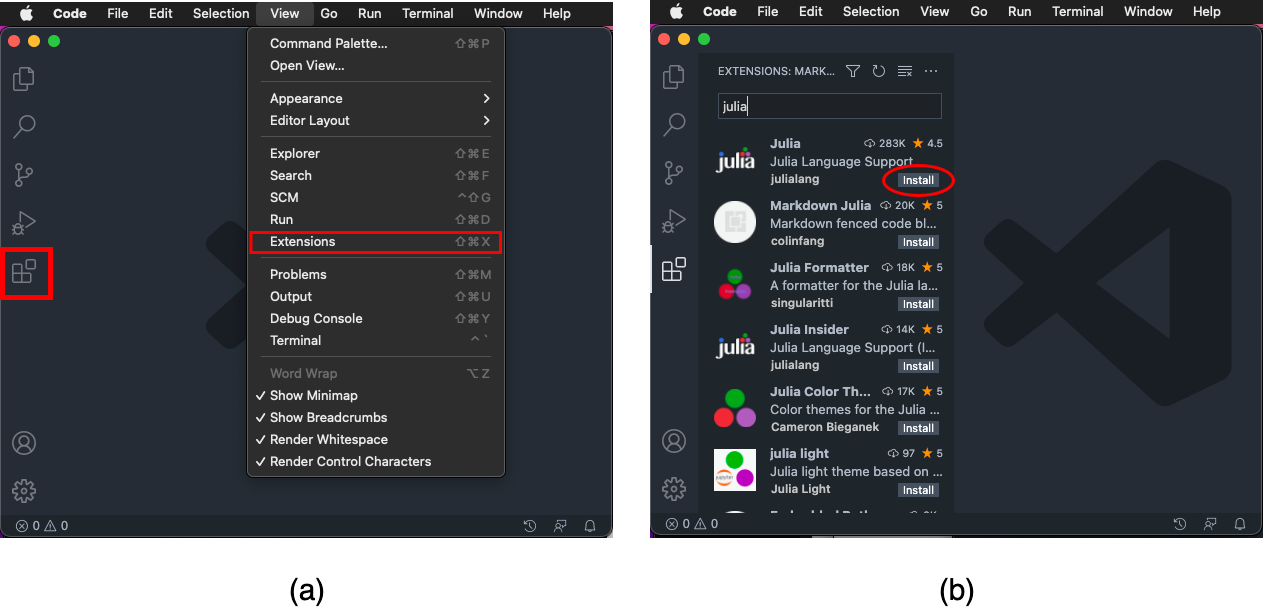
\includegraphics{./images/vscode-extension.png}

}

\caption{\label{fig-vscode-ext}\textbf{Installing Julia extension}.
Figure (a) illustrates the two ways you can access the extension panel.
Figure (b) illustrates how to search and find the Julia extension.}

\end{figure}

This will open-up a panel towards the left side of your VS Code
application; that's your extensions panel. Towards the top of your
extension panel you will see a search box where you have to search for
\texttt{Julia}. In the results, you will see \texttt{Julia} listed as
the top entry. Right next to it, you will also see the \texttt{Install}
button. Click on it. (Figure~\ref{fig-vscode-ext}. b).

\hypertarget{sec-extension-check}{%
\subsection{Checking if the Julia Extension is configured
properly}\label{sec-extension-check}}

In most cases VS Code should be able to automatically configure the path
to julia executable. To check if you have got everything right:

\begin{itemize}
\tightlist
\item
  Do \texttt{Ctrl\ +\ Shift\ +\ P} (Windows) or
  \texttt{Cmd\ +\ Shift\ +\ P} (Mac)
\item
  Type \emph{Start Julia REPL }and hit enter.
\end{itemize}

If a new panel pop-up at the bottom of your VS Code with \texttt{julia}
prompt (as shown below), that means your VS Code Julia extension is
properly configured

\begin{Shaded}
\begin{Highlighting}[]
\NormalTok{julia}\OperatorTok{\textgreater{}}
\end{Highlighting}
\end{Shaded}

\hypertarget{sec-ext-config}{%
\subsection{Fixing the Extension Configuration
Manually}\label{sec-ext-config}}

If you don't get the \texttt{julia} prompt that means VS Code has failed
to automatically configure the path to julia executable. To manually
configure, follow these steps (\emph{also refer to
Figure~\ref{fig-ext-fix}}):

\begin{itemize}
\tightlist
\item
  Open your VS Code extensions panel using any one of the methods
  mentioned above.
\item
  Search for Julia. Now instead of seeing the install button next to
  \texttt{Julia} entry, you will see a gear. Click on it.
\item
  Upon clicking on the gear button, a drop down menu will pop up. Choose
  \texttt{Extension\ Settings} from the list. This will open up the
  setting page.
\item
  In the setting page, you should find a search box at the top. In the
  search box, type \texttt{julia\ executable}
\item
  Now you will see an empty field with the title ``Julia: Executable
  Path''.

  \begin{itemize}
  \tightlist
  \item
    (Windows users): In this field, you need to enter/paste the path you
    copied during step 1 (Section~\ref{sec-install-julia}). (Make sure
    the path ends with
    \texttt{\textbackslash{}bin\textbackslash{}julia.exe}).
  \item
    (Mac users): Run julia from the applications launchpad (just the way
    you open any other application in Mac). Once the Julia application
    is open you will see a path within single quotes right before the
    Julia logo banner. Copy everything between those quotes (excluding
    the quotes) and paste them into the ``Julia: Executable Path'' field
    in VS Code Julia extension.\\
  \end{itemize}
\item
  Close VS Code completely and open it again for the changes to reflect.
\item
  Now repeat the steps mentioned in Section~\ref{sec-extension-check} to
  check if your configuration is working.
\end{itemize}

\begin{figure}

{\centering 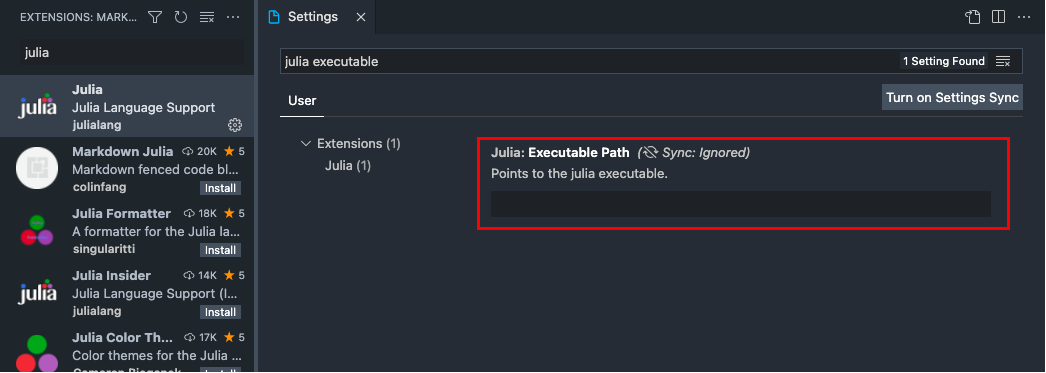
\includegraphics{./images/fix-julia-ext2.png}

}

\caption{\label{fig-ext-fix}\textbf{Configuring Julia extension
manually.} Paste the path you copied during step 1
(Section~\ref{sec-install-julia}) in the textbox area highlighted.}

\end{figure}

\hypertarget{sec-julia-vscode-default}{%
\subsection{Setting Julia as the default language in VS
Code}\label{sec-julia-vscode-default}}

\begin{itemize}
\tightlist
\item
  Follow the instructions described in Section~\ref{sec-ext-config}
  (until step three) to access the extension settings.
\item
  Clear all existing text in the search box of extension setting and
  search for \texttt{default\ language\ mode}.
\item
  In the textbox for \emph{Files: Default Language} that appear, type
  \texttt{julia} (make sure all are lowercase).
\end{itemize}

\hypertarget{know-your-ide}{%
\section{Know Your IDE}\label{know-your-ide}}

IDE stands for Integrated Development Environment and are software that
combine developer tools into a unified user interface. The primary goal
of an IDE is to increase the productivity of the developer by automating
as many redundant configuration steps as possible. Modern IDEs like VS
Code provide functionalities like syntax highlighting (highlights
different component of language in different fonts and color), code
completion (similar to word completion in MS Word), debugging (tools to
debug your code when it is not behaving the way you wanted it to
behave), code search (a local search engine for your project), file
explorer, language terminal (for quick prototyping), and many more
(Figure~\ref{fig-vscode-home}).

\begin{figure}

{\centering 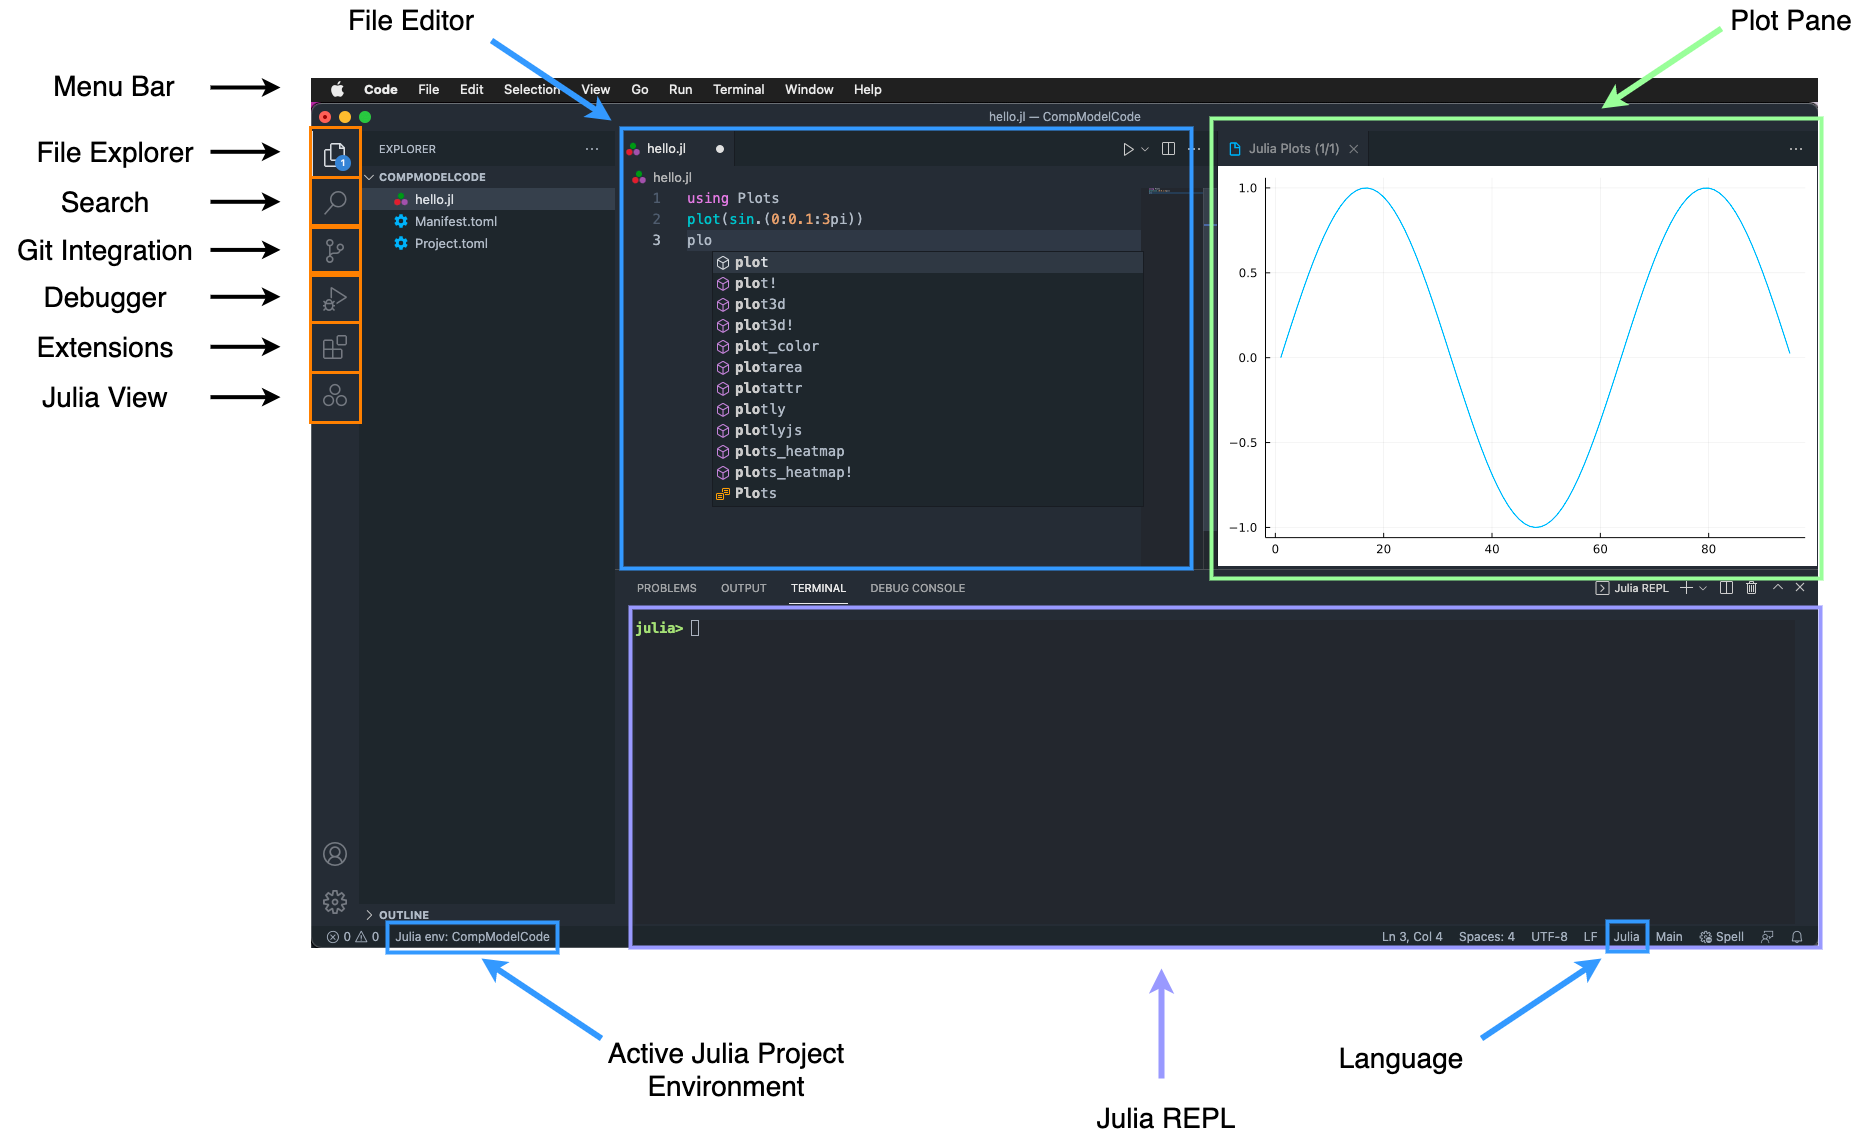
\includegraphics{./images/vscode-tour.png}

}

\caption{\label{fig-vscode-home}Julia VS Code IDE.}

\end{figure}

VS Code, by default, is a simple code/text editor and it is the
extensions (similar to the Julia extension you installed) that bring the
complete IDE experience to VS Code users. Figure~\ref{fig-vscode-home}
provides a visual overview of the VS Code environment during a typical
Julia workflow with an active project environment. To activate the Julia
language environment inside VS Code:

\begin{itemize}
\tightlist
\item
  Do \texttt{Ctrl\ +\ Shift\ +\ P} (Windows) or
  \texttt{Cmd\ +\ Shift\ +\ P} (Mac). This opens the Command Palette
  with a search box.
\item
  Type \texttt{Julia\ REPL} into the search box and hit enter.
\end{itemize}

If the Julia extension is properly configured, the above commands will
open a new terminal with \texttt{julia\textgreater{}} prompt (in most
cases as the bottom panel in VS Code window). This terminal with
\texttt{julia\textgreater{}} prompt is commonly known as the REPL.

\hypertarget{julia-repl}{%
\subsection{Julia REPL}\label{julia-repl}}

REPL stands for Read-Evaluate-Print-Loop and is a method for exploratory
programming and debugging. Julia's REPL provides different prompt modes
and the default one is the Julian (\texttt{julia\textgreater{}}) mode.

\begin{itemize}
\item
  \textbf{Julian Mode.} In julian mode, you can run any julia commands
  and the results will be displayed within the same terminal. It is very
  common among julia programmers to use the julian mode in the REPL to
  try out simple algorithms and ideas. After placing the cursor on the
  REPL, if you press the up arrow or down arrow, you can access your
  REPL history (i.e.~commands you ran in the REPL).
\item
  \textbf{Help Mode.} To access help mode, first place the cursor on the
  REPL and press \texttt{?} in your keyboard. You will see that the
  \texttt{julia\textgreater{}} prompt have changed to
  \texttt{help?\textgreater{}} prompt. This means you are in the help
  mode. Inside the help mode if you type a function name and hit enter,
  julia will attempt to print the documentation associated with that
  function/command in the same terminal.
\item
  \textbf{Package Mode.} Package mode can be accessed from the julian
  mode by pressing \texttt{{]}} key. This will turn the
  \texttt{julia\textgreater{}} prompt to
  \texttt{(@v1.7)\ pkg\textgreater{}} prompt. Package mode is needed for
  installing, updating, and removing julia packages from your projects
  and computer.
\end{itemize}

To return to the default julian mode from one of the other modes, press
backspace.

\hypertarget{sec-install-package}{%
\subsection{Installing Packages}\label{sec-install-package}}

Once you are in the package manager mode you can install a package using
the command \texttt{add}. For e.g., to install the \texttt{StatsBase}
package you'll enter \texttt{add\ StatsBase} into your package manager
mode and hit enter. Once the installation of the package is over, the
prompt will return back to \texttt{(@v1.7)\ pkg}. To remove a package
you use the \texttt{rm} command, and to update a package you use
\texttt{update} command. Just like the \texttt{add} command, you also
need to pass the name of the package in all these cases. You can use the
\texttt{st} command to see the list of packages installed in your
computer/project environment.

\hypertarget{but-what-are-packages}{%
\paragraph{But What are Packages?}\label{but-what-are-packages}}

A Julia package or a library is a collection of functions and
sub-modules surrounding an idea or concept bundled as a single unit.
Each function can be considered as a collection of code whose objective
is to perform a specific task. The standard Julia installation comes
with only a handful of very important packages to get you started. To
extend the capabilities of julia, you install packages with the help of
julia's package manager (Section~\ref{sec-install-package}).

\hypertarget{sec-julia-files}{%
\subsection{Julia Files}\label{sec-julia-files}}

Although you can completely develop julia packages/programs/scripts
within the julia REPL, an easier and faster workflow for developing code
is by writing the commands in a file and running that file in the julia
REPL. To open a new file, do \texttt{Cmd\ +\ N} (Mac) or
\texttt{Ctrl\ +N} (Windows). You can also open a new file using the menu
bar: Choose \texttt{File} --\textgreater{} \texttt{New\ File}. If you
have configured the default language for VS Code as julia
(Section~\ref{sec-julia-vscode-default}), the newly opened file will be
a julia file. It is important for VS Code to know the type of the file
for syntax highlighting, auto code completion and for running the file
in the appropriate language's compiler. Once you have a file open in
your VS Code, you can start writing your code line by line in that file.

\hypertarget{sec-julia-script}{%
\subsection{Running Your First Julia Script}\label{sec-julia-script}}

Suppose you wanted to write a julia script to solve for hypotenuse using
the pythagoras theorem. You know that as per the pythagoras theorem,
\(c = \sqrt{a^2 + b^2}\), where \(c\) is the hypotenuse, and \(a\) and
\(b\) are the sides of a right triangle. You also know that \((3,4,5)\)
is a pythagorean triple. So now let's implement this in code and see if
it gives the right answer.

As a first step you enter the following lines of code into your newly
opened julia file in VS Code:

\begin{Shaded}
\begin{Highlighting}[]
\NormalTok{a }\OperatorTok{=} \FloatTok{3}
\NormalTok{b }\OperatorTok{=} \FloatTok{4}
\NormalTok{c }\OperatorTok{=} \FunctionTok{sqrt}\NormalTok{(a}\OperatorTok{\^{}}\FloatTok{2} \OperatorTok{+}\NormalTok{ b}\OperatorTok{\^{}}\FloatTok{2}\NormalTok{)}
\end{Highlighting}
\end{Shaded}

Now save this file either using \texttt{Cmd\ +\ S} command or
\texttt{File} --\textgreater{} \texttt{Save}. You can give any names you
want, but it is always recommended to use meaningful names (in this
case, say \texttt{pythagoras.jl}) so it is easier to find these files
later. While saving the file also make sure the file have a \texttt{.jl}
extension. Once you have saved the file, you have three ways to run this
script:

\begin{itemize}
\tightlist
\item
  Manually run the script line by line.
\item
  Run the script as a whole.
\item
  Run the file from REPL.
\end{itemize}

To manually run the script line by line, you can place the cursor on the
first line of code and then do \texttt{Shift\ +\ Enter}. If the cursor
hasn't moved automatically to the next line, you can use the down arrow
key to move the cursor to the next line. Now you repeat
\texttt{Shift+Enter} until the last line of code in your file. Once a
line of code is executed, the output of that command is either shown
right next to the command or is printed in the REPL.

To run the script as a whole, you click on the play button you see in
the tab bar of VS Code. While running scripts using this method, only
the output of the last line of code is displayed in the REPL. In our
case, the output will be:

\begin{verbatim}
5.0
\end{verbatim}

To run the file in REPL, you type \texttt{include("YourFileName.jl")}
(in our case \texttt{include("pythagoras.jl")}) into your REPL and hit
enter. The codes' behavior will be similar to the one when you run the
script as a whole using the run button.

\hypertarget{project-environments}{%
\section{Project Environments}\label{project-environments}}

A good programming practice is to always have separate folders for each
Julia project you are working on. However, just having separate folders
isn't going to ensure either reproducibility or an isolated workspace.
(Reproducibility is the property of your project/code to behave exactly
in the same way in a computer other than one in which it was
developed.). To have an isolated workspace, on top of having a separate
folder for your projects, you should also be having what's called
separate project environments (Figure~\ref{fig-proj_env}). Project
environments are like isolated pockets of spaces where your interaction
with one pocket doesn't affect the state of another pocket.

\begin{figure}

{\centering 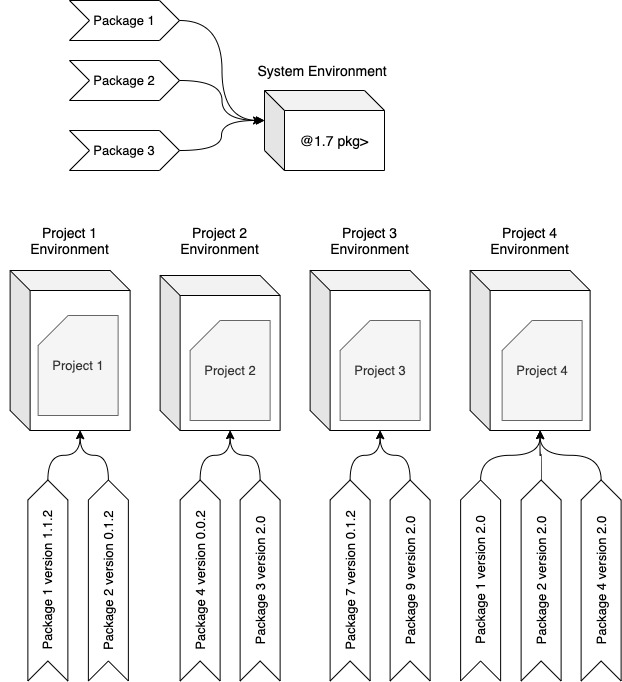
\includegraphics[width=0.55\textwidth,height=\textheight]{./images/project_env.jpg}

}

\caption{\label{fig-proj_env}A schematic diagram to understand the
concept of system environment and project environments.}

\end{figure}

When you install a specific version of Julia, Julia creates an
environment for that particular version. For example, when you installed
Julia 1.7 in your computer, julia also created an environment with the
name 1.7. This is sometimes referred as the global environment or the
system environment. If you didn't activate a particular project's local
environment before staring to work on your project, by default the
system environment will be chosen and all your interaction with the
package manager will be affecting the package state of your Julia's
system environment. For every project environment (including system
environment), Julia creates two files: Manifest.toml and Project.toml.
The goal of these files is to captures the list of packages along with
their version number that you are installing within that environment.

To activate a local environment for your project:

\begin{itemize}
\tightlist
\item
  Open your project folder using VS Code: \texttt{File} --\textgreater{}
  \texttt{Open\ Folder}.
\item
  Now start the Julia REPL using \texttt{Ctrl\ +\ Shift\ +\ P} (or
  \texttt{Cmd\ +\ Shift\ +\ P}).
\item
  Enter package manager mode. If you are seeing \texttt{(@v1.7)\ pkg},
  that means you are in Julia's system environment.
\item
  To create \texttt{\textbackslash{}} activate local environment for
  your project, type \texttt{activate\ .} and hit Enter.
\item
  If your project environment was successfully activated,
  \texttt{(@v1.7)\ pkg} will turn into
  \texttt{(Your\ Folder\ Name)\ pkg}.
\end{itemize}

\hypertarget{your-first-model}{%
\chapter{Your First Model}\label{your-first-model}}

\begin{tcolorbox}[standard jigsaw,bottomtitle=1mm, titlerule=0mm, title={In this chapter you'll learn:}, leftrule=.75mm, toptitle=1mm, arc=.35mm, rightrule=.15mm, opacitybacktitle=0.6, colframe=quarto-callout-caution-color-frame, bottomrule=.15mm, colbacktitle=quarto-callout-caution-color!10!white, colback=white, toprule=.15mm, left=2mm, coltitle=black, opacityback=0]

\begin{enumerate}
\def\labelenumi{\arabic{enumi}.}
\tightlist
\item
  What is machine learning and what are the different types of learning
  algorithms.
\item
  What do you mean by a model in machine learning.
\item
  How to implement a simple model using \texttt{ScikitLearn.jl}
\end{enumerate}

\end{tcolorbox}

\hypertarget{sec-ml}{%
\section{What is Machine Learning?}\label{sec-ml}}

Machine Learning is a sub-field of statistics and optimization where
your goal is to design, develop, and analyze algorithms that can learn
patterns in the data. Algorithms can be thought of as procedures you
need to follow to achieve a goal. Some examples of instances in your
life where you use an algorithm include recipes for food, instructions
for the direction to a place, strategies for solving a math problem,
etc. (Computer algorithms are definitely different from the above
examples, but I hope you got the general gist of what an algorithm
means) Let's take the example of food recipes to understand some
concepts in machine learning further.

Everyone who has learned to cook by themselves knows that the meal isn't
guaranteed to taste that well the first time they try a new recipe. But
with multiple attempts, you learn to adjust the spiciness, sourness,
sweetness, gravy level, etc., to the right proportion that you will be
successful in preparing an outstanding meal. If they were to record each
of their attempts in a table, it would have looked something like this:

\hypertarget{reiepe_data}{}
\begin{table}
\caption{Food ingredients and their proportions.}

\centering
\begin{tabular}{r|ccccccc}
    & Chilly\_Powder & Sugar & Salt & Pepper & Broth\_Oz & Serves & Tastes\\
    \hline
    & Float64 & Int64 & Float64 & Int64 & Float64 & Int64 & String\\
    \hline
    1 & 2.5 & 5 & 0.0 & 3 & 5.0 & 5 & Edible \\
    2 & 1.5 & 4 & 0.5 & 0 & 10.5 & 2 & Average \\
    3 & 2.5 & 4 & 0.0 & 2 & 10.5 & 5 & Non-Edible \\
    4 & 1.0 & 4 & 2.0 & 1 & 11.0 & 1 & Best \\
    5 & 2.0 & 1 & 3.0 & 2 & 5.0 & 5 & Average \\
    6 & 2.0 & 2 & 0.0 & 4 & 6.5 & 3 & Best \\
    7 & 2.0 & 0 & 3.0 & 4 & 12.0 & 4 & Non-Edible \\
    8 & 2.5 & 1 & 0.5 & 1 & 4.5 & 4 & Average \\
    9 & 3.0 & 0 & 1.0 & 4 & 3.0 & 2 & Best \\
    10 & 2.5 & 3 & 1.0 & 4 & 3.0 & 3 & Edible \\
\end{tabular}
\end{table}

\emph{Note: Values in the above table were randomly generated.}

In most cases, a table like the above one is called the data and each of
your attempts (each row) is called an observation. With a data like this
I can do 2 things:

\begin{enumerate}
\def\labelenumi{\arabic{enumi}.}
\tightlist
\item
  Learn how values for each of \texttt{Chilly\_Powder}, \texttt{Sugar},
  \texttt{Salt}, \texttt{Pepper}, \texttt{Broth\_Oz} and \texttt{Serves}
  influence the \texttt{Tastes} and use that information to come up with
  the best combination of values to ensure \texttt{Best} taste all the
  time. This is called \textbf{\emph{inferential modeling}}.
\item
  Given a set of values for \texttt{Chilly\_Powder}, \texttt{Sugar},
  \texttt{Salt}, \texttt{Pepper}, \texttt{Broth\_Oz} and
  \texttt{Serves}, I can predict if the meal is going to be
  \texttt{Edible} or not. This is called \textbf{\emph{predictive
  modeling}}.
\end{enumerate}

If we use the machine learning terminologies, the columns
\texttt{Chilly\_Powder}, \texttt{Sugar}, \texttt{Salt}, \texttt{Pepper},
\texttt{Broth\_Oz} and \texttt{Serves} are called
\textbf{\emph{features}} and the column \texttt{Tastes} is called
\textbf{\emph{target}}. The degree of effect each variable has on the
\texttt{Tastes} are called parameters.

The mathematical representation of the above information in a functional
form is called a \textbf{\emph{model}}. So, for the food recipe example,
our model is:

Chances (Probability) of the meal being edible = \(f(\)
\(\theta_1 \times\) \texttt{Chilly\_Powder} + \(\theta_2 \times\)
\texttt{Sugar} + \(\theta_3 \times\) \texttt{Salt} + \(\theta_4 \times\)
\texttt{Pepper} + \(\theta_5 \times\) \texttt{Broth\_Oz} +
\(\theta_6 \times\) \texttt{Serves} \()\)

\hypertarget{supervised-unsupervised-and-semi-supervised-learning}{%
\subsection{Supervised, Unsupervised, and Semi-supervised
learning}\label{supervised-unsupervised-and-semi-supervised-learning}}

The parameters, \(\theta_1, \theta_2, ....\theta_6\), represent the
patterns in the given dataset and the goal of a Machine Learning
algorithm is to find values for \(\theta_1, \theta_2, ....\theta_6\), so
that I can reliably predict \texttt{Tastes} all the time. This type of
machine learning problem, where I have information about the outcome of
each attempt, is called \textbf{\emph{supervised learning}}.

Suppose in our food recipe example, we didn't have information about if
the meal was edible or not; finding patterns in the data is still
possible. The type of machine learning problem, where I don't have
information about the outcome of each attempt is called
\textbf{\emph{unsupervised learning}}.

Sometimes we use both supervised and unsupervised learning strategy to
solve a problem and those types of machine learning problems are called
\textbf{\emph{semi-supervised learning}}.

Now let's learn how to implement a simple model for a supervised
learning problem similar to the one we discussed above.

\hypertarget{implementing-a-simple-model}{%
\section{Implementing a simple
model}\label{implementing-a-simple-model}}

In this section we'll learn how to implement a simple logistic
regression model to predict if a woman is diabetic or not based on some
of the medical information we have about that person. The dataset we are
using in this section (refer Table~\ref{tbl-pima}) is structurally
similar to the food recipe example we had in the last section. Before
getting into the nitty gritty details of model implementation, let's
learn more about Logistic Regression.

\hypertarget{logistic-regression}{%
\subsection{Logistic Regression}\label{logistic-regression}}

In Section~\ref{sec-ml}, we learned that a model is nothing but a
mathematical representation of the relationship between the features
(aka predictors) and the target. In the diabetes dataset, our target is
the variable that predicts if a person is diabetic or not, and all other
variables are considered features. We can represent this information in
a general form as:

Probability of being diabetic (i.e \texttt{Type} == 1) =

\(f(\)\texttt{NPreg}, \texttt{Glu},\texttt{BP}, \texttt{Skin},
\texttt{BMI}, \texttt{Ped}, \texttt{Age}\() =\)
\[f(\theta_1 \times \text{NPreg} +
\theta_2 \times \text{Glu} +
\theta_3 \times \text{BP} +
\theta_4 \times \text{Skin} +
\] \[
\theta_5 \times \text{BMI} +
\theta_6 \times \text{Ped} +
\theta_7 \times \text{Age}) \tag{1}\]

If we give a logistic parametric form to our function \(f(.)\), then
it's called the logistic regression model. A logistic function is
defined as \[f(x) = \frac{1}{1 + e^{-x}} \tag{2}\]

Using equation \((2)\) on \((1)\) we get,

Probability of being diabetic =
\[\frac{1}{1 + e^{- (\theta_1 \times \text{NPreg} +
\theta_2 \times \text{Glu} +
\theta_3 \times \text{BP} +
\theta_4 \times \text{Skin} +
\theta_5 \times \text{BMI} +
\theta_6 \times \text{Ped} +
\theta_7 \times \text{Age})}} \tag{3}\]

Applying different parametric forms to equation (1) yields you different
machine learning models. For e.g., if we had used an identity function
i.e.~\(f(x) = x\), the model we got is called the linear regression
model (\emph{Note:} Linear Regression models are not used for
classification problems. The type of the problem you are trying to solve
always restricts the type of models you can use.).

By using an activation function where the function will return
\texttt{Yes} if the value we get using equation (3) is greater than or
equal to 0.50 and return \texttt{No} otherwise, we can get prediction
from our model that is comparable to the target in our data. The
discrepancy between our model's prediction and target is called the
\textbf{\emph{prediction error}}.

Once we have a model defined and the data available, the next step is to
use an algorithm to learn optimal values for \(\theta\)'s so that I can
predict values of the target consistently. The step where we use an
algorithm to learn optimal values for \(\theta\)'s is called
\textbf{\emph{model training}} and the data we used for training is
called the \textbf{\emph{training dataset}} in machine learning.

\hypertarget{sec-optimization}{%
\subsection{How do Models learn?}\label{sec-optimization}}

Optimization algorithms are what make model training (learning)
possible. In this section, let's learn how they work from a
birds-eye-view, as explaining the technicalities of how optimization
algorithms work is beyond the scope of this textbook.

\begin{figure}

{\centering 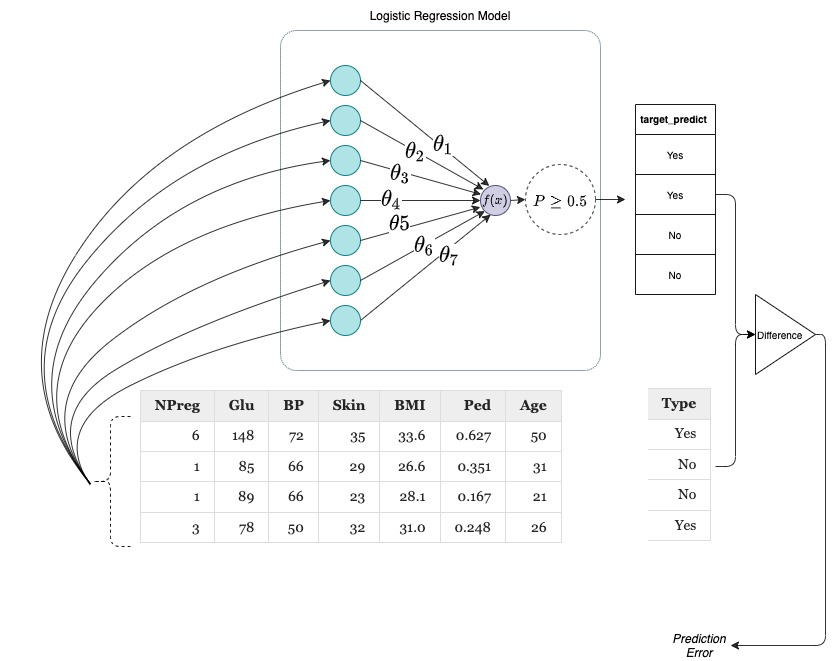
\includegraphics{./images/logisticregression.jpg}

}

\caption{Schematic to understand the concept of model training.}

\end{figure}

An optimization algorithm learns pretty much the same way you learn
things - through trail and error. With each trial, the goal of the
optimization algorithm is to keep reducing the value of prediction error
by manipulating the values for the model parameters (\(\theta\)s). After
several trials, we get to a point where the prediction error is in an
acceptable range and reducing prediction error further is impossible or
futile. At that point, we save the values of \(\theta\) that helped us
to reach that particular prediction error value. These saved values for
\(\theta\) are called the \textbf{\emph{coefficients}} of our learned
model and corresponds to the patterns that were present in our data.
Using the learned coefficients of our model, we will be able to make
predictions on data the model has never seen. The data that the model
hasn't seen is called the \textbf{\emph{test dataset}} and the
prediction error we get on the test data is called the
\textbf{\emph{test error}} and the prediction error we were getting
during training phase is called \textbf{\emph{training error}}.

Now let's learn how to implement a logistic regression model and train
them on the data we have

\hypertarget{step-1-project-environment-activation-and-package-installation}{%
\subsection*{Step 1: Project environment activation and Package
Installation}\label{step-1-project-environment-activation-and-package-installation}}
\addcontentsline{toc}{subsection}{Step 1: Project environment activation
and Package Installation}

\textbf{\emph{Note:}} We expect that you have created a separate folder
for storing all the julia scripts you'll be developing as part of
learning with this textbook. To open your project folder in VS Code, you
can go to Menu --\textgreater{} File --\textgreater{} Open Folder. From
the dialog box that pops up, you can choose the folder you created.

In order to make sure that you are always working in the correct project
environment, have the following 2 lines of code towards beginning of
every julia script you create:

\begin{Shaded}
\begin{Highlighting}[]
\ImportTok{using} \BuiltInTok{Pkg}
\BuiltInTok{Pkg}\NormalTok{.}\FunctionTok{activate}\NormalTok{(}\StringTok{"."}\NormalTok{)}
\end{Highlighting}
\end{Shaded}

\begin{itemize}
\tightlist
\item
  Instructions on how to create a new julia script is described in
  Section~\ref{sec-julia-files} and Section~\ref{sec-julia-script}
\end{itemize}

In this section we will require 3 packages (To learn how to install a
package, refer Section~\ref{sec-install-package}):

\begin{itemize}
\tightlist
\item
  \texttt{RDatasets}: This package provides an easy access to a lot of
  toy datasets in machine learning.
\item
  \texttt{ScikitLearn}: One of the industry standard packages for doing
  machine learning projects. Provides utilities for model definition,
  training, testing, tuning, and much more.
\item
  \texttt{DataFrames}: A package for handling data in tabular form.
\end{itemize}

\hypertarget{step-2-loading-the-packages}{%
\subsection*{Step 2: Loading the
packages}\label{step-2-loading-the-packages}}
\addcontentsline{toc}{subsection}{Step 2: Loading the packages}

To load these packages, you can have the following line of code right
below the code you wrote in step 1:

\begin{Shaded}
\begin{Highlighting}[]
\ImportTok{using} \BuiltInTok{ScikitLearn}\NormalTok{, }\BuiltInTok{RDatasets}\NormalTok{, }\BuiltInTok{DataFrames}
\end{Highlighting}
\end{Shaded}

\begin{itemize}
\tightlist
\item
  If you got an error while running the above line of code, most of the
  time it means one of the three things:

  \begin{enumerate}
  \def\labelenumi{\arabic{enumi}.}
  \tightlist
  \item
    You haven't installed the package that you are trying to load.
  \item
    You are in the wrong project environment. (This is why we highly
    recommend you to follow step 1 every time you create a new julia
    script.)
  \item
    You have typed a wrong package name. The name of all packages in
    Julia are case sensitive.
  \end{enumerate}
\end{itemize}

\hypertarget{step-3-loading-the-dataset}{%
\subsection*{Step 3: Loading the
dataset}\label{step-3-loading-the-dataset}}
\addcontentsline{toc}{subsection}{Step 3: Loading the dataset}

In this example, we will use the \emph{Diabetes in Pima Indian Women
dataset} (available via \texttt{RDatasets}). (Instruction on how to load
a dataset that is available to you are a \texttt{.CSV} file is provided
in the Appendix (\textbf{?@sec-appendix})). To load the dataset and show
the first four observations, enter the following lines of code:

\begin{Shaded}
\begin{Highlighting}[]
\NormalTok{diabetes }\OperatorTok{=} \FunctionTok{dataset}\NormalTok{(}\StringTok{"MASS"}\NormalTok{, }\StringTok{"Pima.te"}\NormalTok{);}
\FunctionTok{first}\NormalTok{(diabetes,}\FloatTok{4}\NormalTok{)}
\end{Highlighting}
\end{Shaded}

\hypertarget{tbl-pima}{}
\begin{table}
\caption{\label{tbl-pima}Diabetes in Pima Indian Women dataset }

\centering
\begin{tabular}{r|cccccccc}
    & NPreg & Glu & BP & Skin & BMI & Ped & Age & Type\\
    \hline
    & Int32 & Int32 & Int32 & Int32 & Float64 & Float64 & Int32 & Cat…\\
    \hline
    1 & 6 & 148 & 72 & 35 & 33.6 & 0.627 & 50 & Yes \\
    2 & 1 & 85 & 66 & 29 & 26.6 & 0.351 & 31 & No \\
    3 & 1 & 89 & 66 & 23 & 28.1 & 0.167 & 21 & No \\
    4 & 3 & 78 & 50 & 32 & 31.0 & 0.248 & 26 & Yes \\
\end{tabular}
\end{table}

\begin{itemize}
\tightlist
\item
  \texttt{dataset} is a function from \texttt{RDatasets} that provide a
  nice interface to load datasets in DataFrames format. The
  \texttt{dataset} function accepts two arguments: the data source, and
  the dataset name. In this case, the name of our dataset was
  \texttt{Pima.te} and the source was \texttt{MASS} package in R.

  \begin{itemize}
  \tightlist
  \item
    \textbf{Trivia:} If you see a word with \texttt{()} ending, then it
    is a function. A function is a collection of commands (several lines
    of codes) sharing a collective single objective. Anything that is
    passed inside \texttt{()} are called arguments. In our example, the
    objective of \texttt{dataset} function was to return the dataset
    (\texttt{Pima.te}) from the source (\texttt{MASS}) we mentioned.
  \end{itemize}
\item
  \texttt{diabetes} is the name we gave to the variable that stores the
  data that was returned from the \texttt{dataset} function. The
  variable name is arbitrary and you can give whatever name you like.
  However, it is always recommended to give meaningful names.
\end{itemize}

\hypertarget{step-4-making-sense-of-the-dataset}{%
\subsection*{Step 4: Making sense of the
dataset}\label{step-4-making-sense-of-the-dataset}}
\addcontentsline{toc}{subsection}{Step 4: Making sense of the dataset}

The diabetes dataset that we are using in this section was collected by
the US National Institute of Diabetes, Digestive, and Kidney Diseases
from a population of women who were 21 years and older and were of Pima
Indian heritage living near Phoenix, Arizona. The dataset contains the
following information:

\begin{itemize}
\tightlist
\item
  \texttt{NPreg}: Number of pregnancies
\item
  \texttt{Glu}: Plasma glucose concentration in an oral glucose
  tolerance test
\item
  \texttt{BP}: Diastolic blood pressure (mm Hg)
\item
  \texttt{Skin}: Triceps skin fold thickness (mm)
\item
  \texttt{BMI}: Body Mass Index
  (\(\frac{\text{weight (Kg)}}{\text{height (m)}^2}\))
\item
  \texttt{Ped}: Diabetic pedigree function
\item
  \texttt{Age}: age in years
\item
  \texttt{Type}: Diabetic or not (according to WHO criteria)
\end{itemize}

\hypertarget{accessing-elements-in-the-data}{%
\subsection*{Accessing elements in the
data}\label{accessing-elements-in-the-data}}
\addcontentsline{toc}{subsection}{Accessing elements in the data}

Now let's take a small detour and learn how to access different cells
and slice the data.

\begin{itemize}
\item
  To access the \(10^\text{th}\) row in the data:

\begin{Shaded}
\begin{Highlighting}[]
\NormalTok{diabetes[}\FloatTok{10}\NormalTok{,}\OperatorTok{:}\NormalTok{]}
\end{Highlighting}
\end{Shaded}

  \hypertarget{tenth_row}{}
  \begin{tabular}{r|cccccccc}
    & NPreg & Glu & BP & Skin & BMI & Ped & Age & Type\\
    \hline
    & Int32 & Int32 & Int32 & Int32 & Float64 & Float64 & Int32 & Cat…\\
    \hline
    10 & 9 & 119 & 80 & 35 & 29.0 & 0.263 & 29 & Yes \\
  \end{tabular}

  \begin{itemize}
  \tightlist
  \item
    The first position in \texttt{{[}{]}} indicated the row, and the
    second position indicated column. If you want to choose all columns
    then you put \texttt{:} in the second position.
  \end{itemize}
\item
  To access the column \texttt{BMI}:
\end{itemize}

\begin{Shaded}
\begin{Highlighting}[]
\NormalTok{diabetes[}\FloatTok{5}\OperatorTok{:}\FloatTok{9}\NormalTok{,}\OperatorTok{:}\NormalTok{BMI]}
\end{Highlighting}
\end{Shaded}

\begin{verbatim}
5-element Vector{Float64}:
 30.5
 25.8
 45.8
 43.3
 39.3
\end{verbatim}

\begin{itemize}
\item
  If you want to choose all rows, then you put \texttt{!} in the first
  position instead of \texttt{5:9}.
\item
  To select multiple columns:
\end{itemize}

\begin{Shaded}
\begin{Highlighting}[]
\NormalTok{diabetes[}\FloatTok{5}\OperatorTok{:}\FloatTok{10}\NormalTok{,[}\OperatorTok{:}\NormalTok{BMI,}\OperatorTok{:}\NormalTok{Age]]}
\end{Highlighting}
\end{Shaded}

\begin{table}
\caption{Accessing multiple columns (for rows from 5:10)}

\centering
\begin{tabular}{r|cc}
    & BMI & Age\\
    \hline
    & Float64 & Int32\\
    \hline
    1 & 30.5 & 53 \\
    2 & 25.8 & 51 \\
    3 & 45.8 & 31 \\
    4 & 43.3 & 33 \\
    5 & 39.3 & 27 \\
    6 & 29.0 & 29 \\
\end{tabular}
\end{table}

\begin{itemize}
\tightlist
\item
  To select all columns except \texttt{Type}:
\end{itemize}

\begin{Shaded}
\begin{Highlighting}[]
\NormalTok{diabetes[}\FloatTok{5}\OperatorTok{:}\FloatTok{10}\NormalTok{,}\FunctionTok{Not}\NormalTok{(}\OperatorTok{:}\DataTypeTok{Type}\NormalTok{)]}
\end{Highlighting}
\end{Shaded}

\begin{table}
\caption{All columns except Type (for rows from 5:10)}

\centering
\begin{tabular}{r|ccccccc}
    & NPreg & Glu & BP & Skin & BMI & Ped & Age\\
    \hline
    & Int32 & Int32 & Int32 & Int32 & Float64 & Float64 & Int32\\
    \hline
    1 & 2 & 197 & 70 & 45 & 30.5 & 0.158 & 53 \\
    2 & 5 & 166 & 72 & 19 & 25.8 & 0.587 & 51 \\
    3 & 0 & 118 & 84 & 47 & 45.8 & 0.551 & 31 \\
    4 & 1 & 103 & 30 & 38 & 43.3 & 0.183 & 33 \\
    5 & 3 & 126 & 88 & 41 & 39.3 & 0.704 & 27 \\
    6 & 9 & 119 & 80 & 35 & 29.0 & 0.263 & 29 \\
\end{tabular}
\end{table}

\hypertarget{step-5-choosing-the-features-and-the-target}{%
\subsection*{Step 5: Choosing the features and the
target}\label{step-5-choosing-the-features-and-the-target}}
\addcontentsline{toc}{subsection}{Step 5: Choosing the features and the
target}

Our goal in this chapter is to define a supervised machine learning
model that can predict if a woman is diabetic or not given their
pregnancy history, glucose level, blood pressure, skin fold thickness,
BMI, diabetic pedigree function, and their age.

If the value we have to predict is a category, that's called a
\textbf{\emph{classification problem }} and if the value we had to
predict was numeric, it's called a \textbf{\emph{regression problem}}.
Both the examples (food recipe and diabetes) we discussed in this
chapter are classification problems. In the food recipe example the
categories of the target were: \texttt{Non-Edible}, \texttt{Edible},
\texttt{Average}, and \texttt{Best}. For the diabetes dataset, the
categories of the target are \texttt{Yes} and \texttt{No} indicating if
a woman is diabetic or not.

We can use the data slicing skills we learned in the previous section to
extract the features and the target from the data:

\begin{Shaded}
\begin{Highlighting}[]
\NormalTok{features }\OperatorTok{=} \FunctionTok{Array}\NormalTok{(diabetes[!, }\FunctionTok{Not}\NormalTok{(}\OperatorTok{:}\DataTypeTok{Type}\NormalTok{)]);}
\NormalTok{target }\OperatorTok{=} \FunctionTok{Array}\NormalTok{(diabetes[!, }\OperatorTok{:}\DataTypeTok{Type}\NormalTok{]);}
\end{Highlighting}
\end{Shaded}

\begin{itemize}
\tightlist
\item
  The first line selects all columns except the \texttt{Type} column and
  saves them as an Array in the variable \texttt{features}
\item
  The second line selects just the \texttt{Type} column and saves them
  as an Array in the variable \texttt{target}
\end{itemize}

\hypertarget{step-6-creating-a-model-instance}{%
\subsection*{Step 6: Creating a Model
Instance}\label{step-6-creating-a-model-instance}}
\addcontentsline{toc}{subsection}{Step 6: Creating a Model Instance}

Logistic regression model is one of the most simple, common, and
baseline model we use for classification problems. To create a logistic
regression model instance, we can import the Logistic Regression
function from \texttt{linear\_models} in \texttt{ScikitLearn} package.

\begin{Shaded}
\begin{Highlighting}[]
\PreprocessorTok{@sk\_import}\NormalTok{ linear\_model}\OperatorTok{:}\NormalTok{ LogisticRegression;}
\NormalTok{simplelogistic }\OperatorTok{=} \FunctionTok{LogisticRegression}\NormalTok{();}
\end{Highlighting}
\end{Shaded}

\begin{itemize}
\tightlist
\item
  The line \texttt{simplelogistic=LogisticRegression()} creates an empty
  logistic regression model object which can store information about the
  model, data, learning algorithm, and learned parameters. The fields
  that are stored in a model object varies depending on the model you
  are defining.
\item
  the variable name \texttt{simplelogistic} is arbitrary and you can
  give whatever name you like.
\item
  If you are going to create another model instance (say a neural
  network model), don't reuse the variable name. It's better to choose a
  different variable name each time you are defining a new model.
\end{itemize}

\hypertarget{step-7-training-your-model}{%
\subsection*{Step 7: Training your
model}\label{step-7-training-your-model}}
\addcontentsline{toc}{subsection}{Step 7: Training your model}

In Section~\ref{sec-optimization}, you learned how an optimization
algorithm helps the model to learn patterns in the data. The
\texttt{fit!} function from \texttt{ScikitLearn} implements that
procedure.

\begin{Shaded}
\begin{Highlighting}[]
\FunctionTok{fit!}\NormalTok{(simplelogistic, features, target);}
\end{Highlighting}
\end{Shaded}

\begin{itemize}
\tightlist
\item
  the \texttt{fit!} function takes three arguments: the model you want
  to train, the features, and the target.

  \begin{itemize}
  \tightlist
  \item
    Whenever you see an exclamation mark in functions, it means that the
    function is mutating (changing) the values of one or more arguments
    passed to that function. In this case \texttt{fit!} function is
    changing the values of \(\theta\), which is part of the model
    definition.
  \end{itemize}
\end{itemize}

Now you have a logistic regression model (\texttt{simplelogistic})
that's trained on Pima diabetes dataset. To see the learned values for
\(\theta\), you can run the following line of code:

\begin{Shaded}
\begin{Highlighting}[]
\NormalTok{simplelogistic.coef\_}
\end{Highlighting}
\end{Shaded}

\begin{verbatim}
1×7 Matrix{Float64}:
 0.138633  0.0373939  -0.00897535  0.0134173  0.0783658  0.921752  0.0190434
\end{verbatim}

You can plug in these values into equation (3) to reliably compute the
probability of a woman being diabetic.

\hypertarget{code-summary-for-chapter-2}{%
\subsection*{Code Summary for Chapter
2}\label{code-summary-for-chapter-2}}
\addcontentsline{toc}{subsection}{Code Summary for Chapter 2}

\begin{Shaded}
\begin{Highlighting}[]
\CommentTok{\# Activating the local project environment }
\ImportTok{using} \BuiltInTok{Pkg}
\BuiltInTok{Pkg}\NormalTok{.}\FunctionTok{activate}\NormalTok{(}\StringTok{"."}\NormalTok{)}

\CommentTok{\# Loading the packages }
\ImportTok{using} \BuiltInTok{ScikitLearn}\NormalTok{, }\BuiltInTok{RDatasets}\NormalTok{, }\BuiltInTok{DataFrames}

\CommentTok{\# Loading the dataset}
\NormalTok{diabetes }\OperatorTok{=} \FunctionTok{dataset}\NormalTok{(}\StringTok{"MASS"}\NormalTok{, }\StringTok{"Pima.te"}\NormalTok{);}
\FunctionTok{first}\NormalTok{(diabetes,}\FloatTok{4}\NormalTok{)}

\CommentTok{\# Choosing the features and target}
\NormalTok{features }\OperatorTok{=} \FunctionTok{Array}\NormalTok{(diabetes[!, }\FunctionTok{Not}\NormalTok{(}\OperatorTok{:}\DataTypeTok{Type}\NormalTok{)])}
\NormalTok{target }\OperatorTok{=} \FunctionTok{Array}\NormalTok{(diabetes[!, }\OperatorTok{:}\DataTypeTok{Type}\NormalTok{])}

\CommentTok{\# Creating a logistic regression model instance }
\PreprocessorTok{@sk\_import}\NormalTok{ linear\_model}\OperatorTok{:}\NormalTok{ LogisticRegression}
\NormalTok{simplelogistic }\OperatorTok{=} \FunctionTok{LogisticRegression}\NormalTok{()}

\CommentTok{\# Training the model }
\FunctionTok{fit!}\NormalTok{(simplelogistic, features, target)}

\CommentTok{\# Viewing the learned parameters }
\NormalTok{simplelogistic.coef\_}
\end{Highlighting}
\end{Shaded}

In the next chapter, we will learn how to check if our trained model is
a good one or not.

\hypertarget{evaluating-your-models-performance}{%
\chapter{Evaluating Your Model's
Performance}\label{evaluating-your-models-performance}}

\begin{tcolorbox}[standard jigsaw,bottomtitle=1mm, titlerule=0mm, title={In this chapter you'll learn:}, leftrule=.75mm, toptitle=1mm, arc=.35mm, rightrule=.15mm, opacitybacktitle=0.6, colframe=quarto-callout-caution-color-frame, bottomrule=.15mm, colbacktitle=quarto-callout-caution-color!10!white, colback=white, toprule=.15mm, left=2mm, coltitle=black, opacityback=0]

\begin{enumerate}
\def\labelenumi{\arabic{enumi}.}
\tightlist
\item
  How to measure how good your model is.
\item
  Different metrics to measure goodness of fit and how to use the
  metrics functions available in \texttt{ScikitLearn}.
\item
  How to interpret the results from metrics functions.
\end{enumerate}

\end{tcolorbox}

\hypertarget{did-our-model-learn-anything}{%
\section{Did our model learn
anything?}\label{did-our-model-learn-anything}}

In the last chapter, we learned how to train our simple model on the
given dataset. But how do we know that our model learned the patterns in
the data? Well, think about the human learning scenario. How do we come
to the conclusion that somebody has learned something?

Through assessments that test their knowledge.

Similarly, we can put our model to test and see how well they perform on
these tests. One of the most common and initial tests you do once you
have a trained model is to check the number of times your model
predicted the target value correctly, i.e., in our case, how many times
our model predicted the women to be diabetic and in fact the women had
diabetes as per our data records. This measure of the percentage number
of times the model predicts the target value correctly is called the
accuracy of the model.

\[\text{Accuracy =} \frac{\text{No. of correct predictions}}{\text{Total no. of predictions}}\]

To compute the accuracy of our model we first need to generate the
predicted values for our target. This can be achieved using the predict
function in \texttt{scikit-learn}.

\begin{Shaded}
\begin{Highlighting}[]
\NormalTok{logistic\_target\_predict }\OperatorTok{=} \FunctionTok{predict}\NormalTok{(simplelogistic,features);}
\end{Highlighting}
\end{Shaded}

\begin{verbatim}
4-element Vector{Any}:
 "Yes"
 "No"
 "No"
 "No"
\end{verbatim}

\begin{itemize}
\tightlist
\item
  \texttt{predict} function has two arguments. The first one is the
  model from which you want the predictions and the second one is the
  data you want to predict on.
\end{itemize}

Once we have the predicted values, we can pass the predicted values and
the target values from our data to the \texttt{accuracy\_score} function
in the \texttt{metrics} module in \texttt{scikit-learn} to compute the
accuracy of our model.

\begin{Shaded}
\begin{Highlighting}[]
\PreprocessorTok{@sk\_import}\NormalTok{ metrics}\OperatorTok{:}\NormalTok{ accuracy\_score}
\FunctionTok{print}\NormalTok{(}\FunctionTok{accuracy\_score}\NormalTok{(target,logistic\_target\_predict))}
\end{Highlighting}
\end{Shaded}

\begin{verbatim}
0.7921686746987951
\end{verbatim}

\begin{itemize}
\tightlist
\item
  \texttt{accuracy\_score} takes two arguments: the true targets (from
  your given dataset) and the predicted values for target (from your
  model).
\end{itemize}

\begin{itemize}
\tightlist
\item
  The results show that our model has an accuracy of 79.22 \%.
\end{itemize}

\hypertarget{is-our-model-confused}{%
\section{Is our model confused?}\label{is-our-model-confused}}

Although accuracy is a good measure to assess the quality of your model,
most often, especially in classification type problems, they don't tell
us the complete story.

When we do prediction in a classification task, there arise four
situations. For example, in our case:

\begin{itemize}
\tightlist
\item
  the model predicted the woman to be diabetic and was in fact diabetic
\item
  the model predicted the woman to be non-diabetic but was diabetic
\item
  the model predicted the woman to be diabetic but was not actually
  diabetic
\item
  the model predicted the woman to be non-diabetic and was not diabetic
\end{itemize}

The first and last cases where our predictions aligned with the actual
values are called \emph{true positives} and \emph{true negatives}
respectively. The case where the model predicted the woman to be
diabetic while she did not have diabetes is called a \emph{false
positive} case, and the case where the model predicted the woman to be
non-diabetic but she was in fact diabetic is called the
\emph{false-negative} case. This is illustrated in
Figure~\ref{fig-confusion}.

\begin{figure}

{\centering 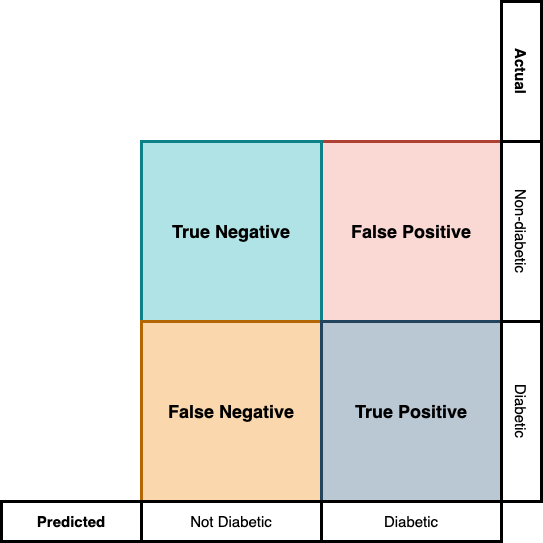
\includegraphics{./images/confusion.png}

}

\caption{\label{fig-confusion}Four possible scenarios in the diabetes
prediction task.}

\end{figure}

When we just focus on a classification model's accuracy, all these
information is hidden from us.

It is possible to generate a figure like Figure~\ref{fig-confusion} in
\texttt{scikit-learn}. For that, you need two functions, the
\texttt{confusion\_matrix} function to generate the confusion matrix and
\texttt{ConfusionMatrixDisplay} function to generate the plot.

\begin{Shaded}
\begin{Highlighting}[]
\CommentTok{\# Generating the confusion matrix }
\PreprocessorTok{@sk\_import}\NormalTok{ metrics}\OperatorTok{:}\NormalTok{ confusion\_matrix}
\NormalTok{cf }\OperatorTok{=} \FunctionTok{confusion\_matrix}\NormalTok{(target, logistic\_target\_predict)}

\CommentTok{\# Loading the plotting library \& confusion matrix plotting function}
\ImportTok{using} \BuiltInTok{PyPlot}
\PreprocessorTok{@sk\_import}\NormalTok{ metrics}\OperatorTok{:}\NormalTok{ ConfusionMatrixDisplay}

\FunctionTok{figure}\NormalTok{() }\CommentTok{\# Open a new canvas to plot}

\CommentTok{\# Generating the plot }
\NormalTok{disp }\OperatorTok{=} \FunctionTok{ConfusionMatrixDisplay}\NormalTok{(confusion\_matrix}\OperatorTok{=}\NormalTok{cf,}
\NormalTok{            display\_labels}\OperatorTok{=}\NormalTok{simplelogistic.classes\_)}
\NormalTok{disp.}\FunctionTok{plot}\NormalTok{() }\CommentTok{\# Transferring the plot to the canvas}
\FunctionTok{gcf}\NormalTok{() }\CommentTok{\# Freezing the canvas and printing it.}
\end{Highlighting}
\end{Shaded}

\hypertarget{why-our-models-confusion-pattern-matters}{%
\section{Why our model's confusion pattern
matters?}\label{why-our-models-confusion-pattern-matters}}

You might still be thinking why these false rates and true rates matter
since we already have the accuracy scores. The importance of the
confusion matrix comes into play when we consider the consequences of
our prediction. For example, if it's a high consequence situation like
predicting if somebody has early-stage cancer or not, miss-classifying a
person as not having cancer, while they have cancer has a high cost. In
such cases, the ML designer needs to look at the false negative rate
more closely than the model's overall accuracy. Whereas, in a low
consequence situation like credit card approval prediction, the false
positive rate matters more than the false negative rate. Because, with
higher false negative rate, you might be denying a credit card to a
person with a good credit score and fewer chances of defaulting whereas
if you have high false positive rate, you will be approving credit cards
to people whose chances of defaulting are high.

The measure we are interested in the first case where the cost of
missing a positive is high is called the recall or sensitivity of our
model. Recall can be computed from your confusion matrix using the
formulae:

\[ \text{Recall =} \frac{\text{True Positives}}{\text{True Positives + False Negatives}}\]

\begin{Shaded}
\begin{Highlighting}[]
\NormalTok{true\_neg, false\_neg, false\_pos, true\_pos }\OperatorTok{=}\NormalTok{ cf}
\NormalTok{recall }\OperatorTok{=}\NormalTok{ true\_pos }\OperatorTok{/}\NormalTok{ (true\_pos }\OperatorTok{+}\NormalTok{ false\_neg)}
\end{Highlighting}
\end{Shaded}

\begin{verbatim}
0.5688073394495413
\end{verbatim}

The measure we are interested in the second case, where the cost of
false positive is higher is called the precision of our model. Precision
can be computed using the formula:

\[\text{Precision =} \frac{\text{True Positives}}{\text{True Positives + False Positives}}\]

\begin{Shaded}
\begin{Highlighting}[]
\NormalTok{precision }\OperatorTok{=}\NormalTok{ true\_pos }\OperatorTok{/}\NormalTok{ (true\_pos }\OperatorTok{+}\NormalTok{ false\_pos)}
\end{Highlighting}
\end{Shaded}

\begin{verbatim}
0.7380952380952381
\end{verbatim}

The above results say that our model has high chances of missing a
diabetes patient (due to low recall) and low chances of generating a
false positive (high precision). In other words, if the model predicted
you as having diabetes, there is a high chance you have diabetes, but if
you were diagnosed non-diabetic by the model, you may or may not be
diabetic.

If your model is used in a scenario where both false positives and false
negatives have high consequences, a better metric to watch for is the F1
score. F1 score is also a better metric than accuracy score for
evaluating model's performance when you have imbalances dataset
(Imbalanced datasets are datasets that have unequal number of data
points across its classes. For e.g., our diabetic dataset will be an
imbalanced data if 90\% of our data are that of non-diabetic people and
only 10\% is that of diabetic people.). F1 score is the weighted average
of precision and recall and can be computed using the formula:

\[\text{F1 score = } 2 \times \frac{\text{Recall} \times \text{Precision}}{\text{Precision + Recall}}\]

\begin{Shaded}
\begin{Highlighting}[]
\NormalTok{f1 }\OperatorTok{=}\NormalTok{ (}\FloatTok{2} \OperatorTok{*}\NormalTok{ precision }\OperatorTok{*}\NormalTok{ recall) }\OperatorTok{/}\NormalTok{ (precision }\OperatorTok{+}\NormalTok{ recall)}
\end{Highlighting}
\end{Shaded}

\begin{verbatim}
0.6424870466321243
\end{verbatim}

Although we had very good accuracy score, the F1 score for our model
suggests that our model isn't that impressive.

To compute the recall, precision, f1 score, and accuracy with lesser
lines of code, you can use the \texttt{classification\_report} function
from \texttt{metrics} module in \texttt{scikit-learn}.

\begin{Shaded}
\begin{Highlighting}[]
\PreprocessorTok{@sk\_import}\NormalTok{ metrics}\OperatorTok{:}\NormalTok{ classification\_report}
\FunctionTok{print}\NormalTok{(}\FunctionTok{classification\_report}\NormalTok{(target, logistic\_target\_predict))}
\end{Highlighting}
\end{Shaded}

\begin{verbatim}
              precision    recall  f1-score   support

          No       0.81      0.90      0.85       223
         Yes       0.74      0.57      0.64       109

    accuracy                           0.79       332
   macro avg       0.77      0.74      0.75       332
weighted avg       0.79      0.79      0.78       332
\end{verbatim}

\begin{itemize}
\tightlist
\item
  The first line list the precision, recall, and f1 score with respect
  to the target ``No'' and the second with respect to the target
  ``Yes''.
\item
  In the above computations, we have calculated precision, recall, and
  f1 score with respect to the target ``Yes''. You can check the values
  we have got manually with the values printed in the classification
  report.
\end{itemize}

\hypertarget{code-summary-for-chapter-3}{%
\section*{Code Summary for Chapter 3}\label{code-summary-for-chapter-3}}
\addcontentsline{toc}{section}{Code Summary for Chapter 3}

\begin{Shaded}
\begin{Highlighting}[]
\CommentTok{\# Generating the predictions from the trained model}
\NormalTok{logistic\_target\_predict }\OperatorTok{=} \FunctionTok{predict}\NormalTok{(simplelogistic,features);}

\CommentTok{\# Calculating the accuracy score }
\PreprocessorTok{@sk\_import}\NormalTok{ metrics}\OperatorTok{:}\NormalTok{ accuracy\_score}
\FunctionTok{print}\NormalTok{(}\FunctionTok{accuracy\_score}\NormalTok{(target,logistic\_target\_predict))}

\CommentTok{\# Generating the confusion matrix }
\PreprocessorTok{@sk\_import}\NormalTok{ metrics}\OperatorTok{:}\NormalTok{ confusion\_matrix}
\NormalTok{cf }\OperatorTok{=} \FunctionTok{confusion\_matrix}\NormalTok{(target, logistic\_target\_predict)}

\CommentTok{\# Loading the plotting library \& confusion matrix plotting function}
\ImportTok{using} \BuiltInTok{PyPlot}
\PreprocessorTok{@sk\_import}\NormalTok{ metrics}\OperatorTok{:}\NormalTok{ ConfusionMatrixDisplay}

\FunctionTok{figure}\NormalTok{() }\CommentTok{\# Open a new canvas to plot}

\CommentTok{\# Generating the plot }
\NormalTok{disp }\OperatorTok{=} \FunctionTok{ConfusionMatrixDisplay}\NormalTok{(confusion\_matrix}\OperatorTok{=}\NormalTok{cf,}
\NormalTok{            display\_labels}\OperatorTok{=}\NormalTok{simplelogistic.classes\_)}
\NormalTok{disp.}\FunctionTok{plot}\NormalTok{() }\CommentTok{\# Transferring the plot to the canvas}
\FunctionTok{gcf}\NormalTok{() }\CommentTok{\# Freezing the canvas and printing it.}

\CommentTok{\# Generating the classification report}
\PreprocessorTok{@sk\_import}\NormalTok{ metrics}\OperatorTok{:}\NormalTok{ classification\_report}
\FunctionTok{print}\NormalTok{(}\FunctionTok{classification\_report}\NormalTok{(target, logistic\_target\_predict))}
\end{Highlighting}
\end{Shaded}

\hypertarget{generalizability}{%
\chapter{Generalizability}\label{generalizability}}

\begin{tcolorbox}[standard jigsaw,bottomtitle=1mm, titlerule=0mm, title={In this chapter you'll learn:}, leftrule=.75mm, toptitle=1mm, arc=.35mm, rightrule=.15mm, opacitybacktitle=0.6, colframe=quarto-callout-caution-color-frame, bottomrule=.15mm, colbacktitle=quarto-callout-caution-color!10!white, colback=white, toprule=.15mm, left=2mm, coltitle=black, opacityback=0]

\begin{enumerate}
\def\labelenumi{\arabic{enumi}.}
\tightlist
\item
  What is generalizability.
\item
  How to ensure generaziability of your model.
\item
  What you mean by learning curve, under-fitting, over-fitting, bias and
  variance.
\item
  How to implement cross-validation techniques using
  \texttt{ScikitLearn}.
\end{enumerate}

\end{tcolorbox}

\hypertarget{did-our-model-cheat}{%
\section{Did our model cheat?}\label{did-our-model-cheat}}

In the last chapter, we learned how to check our model's performance
using various metrics. But how do we know that our model really learned
the patterns in the data and is not cheating by rote-memorizing the
data? Think about how we would have assessed a human learner in this
situation.

When we want to know if students have really learned what we have asked
them to learn, we test students on material that is similar to the
material that's familiar to them but not exactly the questions they have
seen before. Similarly, to check if our models have really learned the
patterns in the data, we can test our model against a similar but unseen
data. The extent to which the model performance remains invariant with
this new unseen data is called that model's
\textbf{\emph{generalizability}}.

The portion of the data we use for training is called the
\textbf{\emph{training set}} and the portion of the data we use to test
is called the \textbf{\emph{test set}}. We can use the
\texttt{train\_test\_split} function from \texttt{model\_selection}
module in \texttt{scikit-learn} to create this partition.

\begin{Shaded}
\begin{Highlighting}[]
\PreprocessorTok{@sk\_import}\NormalTok{ model\_selection}\OperatorTok{:}\NormalTok{ train\_test\_split;}
\NormalTok{features\_train, features\_test, }
\NormalTok{    target\_train, target\_test }\OperatorTok{=} \FunctionTok{train\_test\_split}\NormalTok{(features, }
\NormalTok{        target, test\_size}\OperatorTok{=}\FloatTok{0.3}\NormalTok{, random\_state}\OperatorTok{=}\FloatTok{42}\NormalTok{);}
\end{Highlighting}
\end{Shaded}

\begin{itemize}
\tightlist
\item
  The \texttt{train\_test\_split} function has three important and
  mandatory arguments.
\item
  The first two are the \texttt{features} and the \texttt{target}
\item
  The third argument is \texttt{test\_size} and specifies the proportion
  of the data that needs to kept aside for testing. In the above code,
  we have asked to keep aside 30\% of the data as test set.\\
\item
  \texttt{random\_state} is an optional argument and set's the seed for
  randomness.
\end{itemize}

Now, instead of training the model on the entire dataset, we'll train
our model with training set.

\begin{Shaded}
\begin{Highlighting}[]
\PreprocessorTok{@sk\_import}\NormalTok{ linear\_model}\OperatorTok{:}\NormalTok{ LogisticRegression;}
\NormalTok{simplelogistic }\OperatorTok{=} \FunctionTok{LogisticRegression}\NormalTok{();}

\FunctionTok{fit!}\NormalTok{(simplelogistic, features\_train, target\_train);}
\end{Highlighting}
\end{Shaded}

Now let's look at our model's performance with both training set and
test set.

\hypertarget{in-sample-performance}{%
\subsection*{In-sample performance}\label{in-sample-performance}}
\addcontentsline{toc}{subsection}{In-sample performance}

A model's performance with training set is also called it's in-sample
performance.

\begin{Shaded}
\begin{Highlighting}[]
\NormalTok{logistic\_target\_predict\_training }\OperatorTok{=} 
    \FunctionTok{predict}\NormalTok{(simplelogistic,features\_train);}

\PreprocessorTok{@sk\_import}\NormalTok{ metrics}\OperatorTok{:}\NormalTok{ classification\_report}
\FunctionTok{print}\NormalTok{(}\FunctionTok{classification\_report}\NormalTok{(target\_train,}
\NormalTok{                     logistic\_target\_predict\_training))}
\end{Highlighting}
\end{Shaded}

\begin{verbatim}
              precision    recall  f1-score   support

          No       0.84      0.91      0.87       166
         Yes       0.71      0.56      0.63        66

    accuracy                           0.81       232
   macro avg       0.78      0.74      0.75       232
weighted avg       0.80      0.81      0.80       232
\end{verbatim}

\hypertarget{out-of-sample-performance}{%
\subsection*{Out-of-sample
performance}\label{out-of-sample-performance}}
\addcontentsline{toc}{subsection}{Out-of-sample performance}

A model's performance with test set is also called it's out-of-sample
performance.

\begin{Shaded}
\begin{Highlighting}[]
\NormalTok{logistic\_target\_predict\_test }\OperatorTok{=} 
    \FunctionTok{predict}\NormalTok{(simplelogistic,features\_test);}

\PreprocessorTok{@sk\_import}\NormalTok{ metrics}\OperatorTok{:}\NormalTok{ classification\_report}
\FunctionTok{print}\NormalTok{(}\FunctionTok{classification\_report}\NormalTok{(target\_test,}
\NormalTok{                     logistic\_target\_predict\_test))}
\end{Highlighting}
\end{Shaded}

\begin{verbatim}
              precision    recall  f1-score   support

          No       0.72      0.98      0.83        57
         Yes       0.95      0.49      0.65        43

    accuracy                           0.77       100
   macro avg       0.84      0.74      0.74       100
weighted avg       0.82      0.77      0.75       100
\end{verbatim}

By comparing our model's performance with both the training set and test
set, we can see that the overall accuracy of our model slightly dropped
for the test case. We can also see that our model had better precision
but a little worse recall and f1-score with the test performance
compared to training performance. So, we can conclude that our model has
an ok-ish generalizability.

\hypertarget{cross-validation-a-robust-measure-of-generalizability}{%
\section{Cross-validation: A robust measure of
generalizability}\label{cross-validation-a-robust-measure-of-generalizability}}

We can extend the concepts of in-sample and out-of sample performance to
create a more robust measure of generalizability. There are two
motivations for creating this new robust measure of generalizability:

\begin{enumerate}
\def\labelenumi{\arabic{enumi}.}
\tightlist
\item
  When the sample size is small (less data), our training and test
  performance scores can get flaky and unreliable.
\item
  There are some bells and whistles (which are called hyperparameters)
  that we can tweak in our models to improve our models' learning
  process (This is explained in detail in the coming chapters). If we
  tweak these hyperparameters with respect to our training data, we
  might be overfitting our data to the training set
  (\textbf{\emph{Overfitting}} happens when our model have high
  performance on training set but very poor performance on test set.).
  But instead, if we tweak these hyperparameters with respect to our
  test data, information in the test data leaks to the model and the
  data is no more unseen data for the model.
\end{enumerate}

ML developers came up with a solution to this problem by partitioning
the training data into different data blocks, holding out one block as
test set, and training on the remaining blocks. Then model's performance
on the hold-out test set is saved. This process is repeated until all
blocks had its chance of beginning the hold-out test set. Model
performance from all these iterations is then averaged to get the robust
generalization performance. This process of deriving model performance
is called the \textbf{\emph{cross-validation}} technique and is
illustrated in Figure~\ref{fig-cross-val}.

\begin{figure}

{\centering 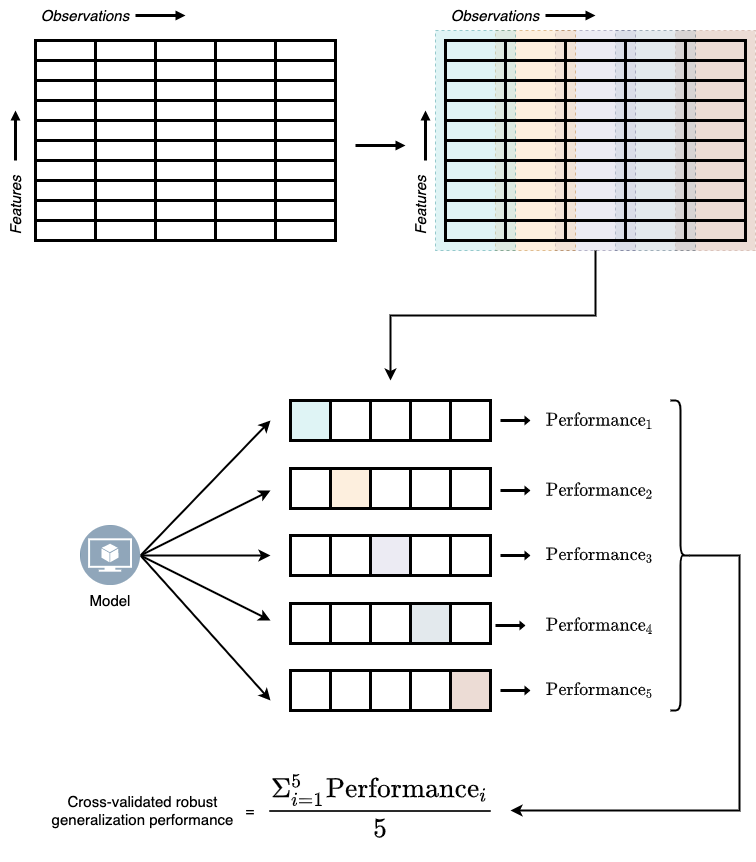
\includegraphics{./images/cross_val.png}

}

\caption{\label{fig-cross-val}Five-fold cross validation}

\end{figure}

To implement the K-fold cross validation technique we can use the
\texttt{KFold} function and \texttt{cross\_validate} function
\texttt{model\_selection} module in \texttt{scikit-learn}.

\begin{Shaded}
\begin{Highlighting}[]
\PreprocessorTok{@sk\_import}\NormalTok{ model\_selection}\OperatorTok{:}\NormalTok{ KFold}
\PreprocessorTok{@sk\_import}\NormalTok{ model\_selection}\OperatorTok{:}\NormalTok{ cross\_validate}

\NormalTok{cv\_results }\OperatorTok{=} \FunctionTok{cross\_validate}\NormalTok{(simplelogistic, }
\NormalTok{        features\_train, target\_train, }
\NormalTok{            cv}\OperatorTok{=}\FunctionTok{KFold}\NormalTok{(}\FloatTok{5}\NormalTok{),}
\NormalTok{            return\_estimator}\OperatorTok{=}\ConstantTok{true}\NormalTok{,}
\NormalTok{            return\_train\_score}\OperatorTok{=}\ConstantTok{true}\NormalTok{, }
\NormalTok{            scoring}\OperatorTok{=}\NormalTok{[}\StringTok{"accuracy"}\NormalTok{,}
                 \StringTok{"recall\_weighted"}\NormalTok{, }\StringTok{"precision\_weighted"}\NormalTok{]);}
\end{Highlighting}
\end{Shaded}

\begin{itemize}
\tightlist
\item
  \texttt{cross\_validate} function has three mandatroy arguments: the
  model, features, and the target. By default \texttt{cross\_validate}
  uses 5-folds for cross validation.
\item
  If you are interested in measures other than accuracy, you can pass
  the list of metrics with \texttt{scoring} argument.
\end{itemize}

To print the results from cross validation in a more human readable
table form, we can use the following lines of code:

\begin{Shaded}
\begin{Highlighting}[]
\NormalTok{cv\_df }\OperatorTok{=} \FunctionTok{DataFrame}\NormalTok{(cv\_results)[!, }
        \FunctionTok{Not}\NormalTok{([}\OperatorTok{:}\NormalTok{estimator, }\OperatorTok{:}\NormalTok{fit\_time, }\OperatorTok{:}\NormalTok{score\_time])]}

\FunctionTok{rename!}\NormalTok{(cv\_df, [}\StringTok{"Test Accuracy"}\NormalTok{,}
                \StringTok{"Test Precision"}\NormalTok{,}
                \StringTok{"Test Recall"}\NormalTok{,}
                \StringTok{"Train Accuracy"}\NormalTok{,}
                \StringTok{"Train Precision"}\NormalTok{,}
                \StringTok{"Train Recall"}\NormalTok{])}
\end{Highlighting}
\end{Shaded}

\begin{tabular}{r|cccccc}
    & Test Accuracy & Test Precision & Test Recall & Train Accuracy & Train Precision & Train Recall\\
    \hline
    & Float64 & Float64 & Float64 & Float64 & Float64 & Float64\\
    \hline
    1 & 0.829787 & 0.818237 & 0.829787 & 0.837838 & 0.833854 & 0.837838 \\
    2 & 0.808511 & 0.801009 & 0.808511 & 0.8 & 0.792456 & 0.8 \\
    3 & 0.76087 & 0.742992 & 0.76087 & 0.811828 & 0.804097 & 0.811828 \\
    4 & 0.847826 & 0.851999 & 0.847826 & 0.811828 & 0.805028 & 0.811828 \\
    5 & 0.782609 & 0.782609 & 0.782609 & 0.817204 & 0.808555 & 0.817204 \\
\end{tabular}

To compute the cross validated average model performance measures, we
can print the mean of each column in the above table.

\begin{Shaded}
\begin{Highlighting}[]
\FunctionTok{describe}\NormalTok{(cv\_df)[!,[}\OperatorTok{:}\NormalTok{variable, }\OperatorTok{:}\NormalTok{mean]]}
\end{Highlighting}
\end{Shaded}

\begin{table}
\caption{Cross validated average model performance measures}

\centering
\begin{tabular}{r|cc}
    & variable & mean\\
    \hline
    & Symbol & Float64\\
    \hline
    1 & Test Accuracy & 0.80592 \\
    2 & Test Precision & 0.799369 \\
    3 & Test Recall & 0.80592 \\
    4 & Train Accuracy & 0.81574 \\
    5 & Train Precision & 0.808798 \\
    6 & Train Recall & 0.81574 \\
\end{tabular}
\end{table}

\begin{itemize}
\tightlist
\item
  \texttt{describe} is a function from \texttt{DataFrames} package that
  returns summary statistics like mean, mode, median, minimum value,
  maximum value, etc., for a given dataframe. We can use this function
  to otain the mean values for our performance measures.
\end{itemize}

\hypertarget{learning-curves-can-more-data-improve-model-training}{%
\section{Learning curves: Can more data improve model
training?}\label{learning-curves-can-more-data-improve-model-training}}

Now we know how to measure a model's generalization performance. But
what if our models perform poorly in both training and test sets? The
scenario where models fit poorly with training and test sets equally is
called \textbf{\emph{underfitting}}. Underfitting usually happens due to
one of the two reasons or both: a) our model is too simple for the task
at hand, b) we don't have enough data to learn from.

Solving the first problem is relatively simple; we can train a more
complex model on the given dataset. However, solving the second problem
can get complicated. Gathering more data may not always be feasible and
can be expensive. In such cases, before deciding on acquiring more data,
we need to make sure more data will solve the problem of underfitting.

The way we figure out if more data can help with training is by training
our model with data of different sizes (e.g., using 10\%, 50\%, and
100\% of our data) and check how the model performance is varying as a
function of the sample size. The plot that illustrates this relationship
is called \textbf{\emph{learning curves}}.

We can get our model's performance at different sample sizes using the
\texttt{learning\_curve} function from \texttt{model\_selection} module
in \texttt{scikit-learn}.

\begin{Shaded}
\begin{Highlighting}[]
\PreprocessorTok{@sk\_import}\NormalTok{ model\_selection}\OperatorTok{:}\NormalTok{ learning\_curve;}
\NormalTok{lc\_results }\OperatorTok{=} \FunctionTok{learning\_curve}\NormalTok{(simplelogistic, }
\NormalTok{        features\_train,target\_train, }
\NormalTok{            train\_sizes }\OperatorTok{=}\NormalTok{ [}\FloatTok{0.06}\NormalTok{, }\FloatTok{0.1}\NormalTok{, }\FloatTok{0.25}\NormalTok{, }\FloatTok{0.5}\NormalTok{, }\FloatTok{0.75}\NormalTok{, }\FloatTok{1.0}\NormalTok{]);}
\end{Highlighting}
\end{Shaded}

\begin{itemize}
\tightlist
\item
  The values we pass to \texttt{train\_sizes} argument specify the
  different sample sizes we want to try. In this case we are looking at
  10\%, 25\%, 50\%, 75\% and 100\% of the data.
\end{itemize}

\begin{Shaded}
\begin{Highlighting}[]
\NormalTok{train\_sizes, train\_scores, test\_scores, }\OperatorTok{=} 
\NormalTok{    lc\_results[}\FloatTok{1}\NormalTok{], lc\_results[}\FloatTok{2}\NormalTok{], lc\_results[}\FloatTok{3}\NormalTok{]}

\ImportTok{using} \BuiltInTok{Statistics}
\CommentTok{\# Calculating the error bars }
\NormalTok{y\_ax }\OperatorTok{=} \FunctionTok{vec}\NormalTok{(}\FunctionTok{mean}\NormalTok{(test\_scores, dims}\OperatorTok{=}\FloatTok{2}\NormalTok{)) }
\NormalTok{y\_err }\OperatorTok{=} \FunctionTok{vec}\NormalTok{(}\FunctionTok{std}\NormalTok{(test\_scores, dims}\OperatorTok{=}\FloatTok{2}\NormalTok{))}

\ImportTok{using} \BuiltInTok{PyPlot}
\ControlFlowTok{begin} 
    \FunctionTok{figure}\NormalTok{();}
    \FunctionTok{plot}\NormalTok{(train\_sizes,}
        \FunctionTok{vec}\NormalTok{(}\FunctionTok{mean}\NormalTok{(test\_scores, dims}\OperatorTok{=}\FloatTok{2}\NormalTok{)), label}\OperatorTok{=}\StringTok{"Cross Val"}\NormalTok{);}

    \FunctionTok{fill\_between}\NormalTok{(train\_sizes,}
\NormalTok{        y\_ax }\OperatorTok{{-}}\NormalTok{ y\_err, y\_ax }\OperatorTok{+}\NormalTok{ y\_err,alpha}\OperatorTok{=}\FloatTok{0.2}\NormalTok{);}

    \FunctionTok{plot}\NormalTok{(train\_sizes,}
        \FunctionTok{vec}\NormalTok{(}\FunctionTok{mean}\NormalTok{(train\_scores, dims}\OperatorTok{=}\FloatTok{2}\NormalTok{)), label}\OperatorTok{=}\StringTok{"Training"}\NormalTok{);}
    \FunctionTok{xlabel}\NormalTok{(}\StringTok{"Training Size"}\NormalTok{); }
    \FunctionTok{ylabel}\NormalTok{(}\StringTok{"Score"}\NormalTok{); }
    \FunctionTok{title}\NormalTok{(}\StringTok{"Learning Curve"}\NormalTok{);}
    \FunctionTok{legend}\NormalTok{(loc}\OperatorTok{=}\FloatTok{4}\NormalTok{);}
    \FunctionTok{gcf}\NormalTok{()}
\ControlFlowTok{end}\NormalTok{;}
\end{Highlighting}
\end{Shaded}

\begin{figure}

{\centering 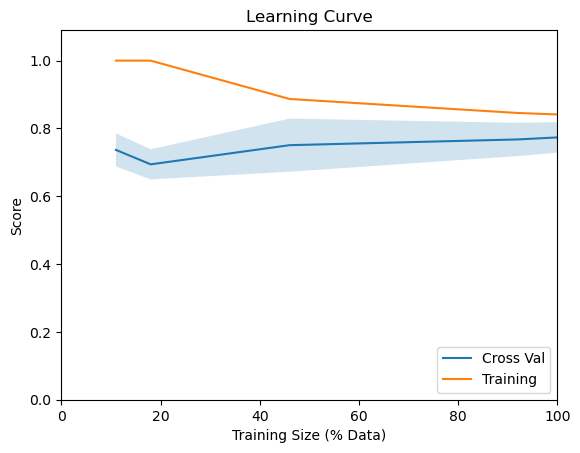
\includegraphics{./generalizability_files/figure-pdf/fig-learning-curve-output-1.png}

}

\caption{\label{fig-learning-curve}Learning Curve for simple logistic
regression model on diabetes dataset}

\end{figure}

From the above learning curve, we see that our model's accuracy isn't
getting that much influenced by increasing the sample size. So, it will
be futile to collect more data for our diabetes detection ML system.
However, if the blue line in Figure~\ref{fig-learning-curve} had a
steeper upward trend, it would have made sense to collect more data to
improve our model's performance.

\hypertarget{code-summary-for-chapter-4}{%
\subsection*{Code Summary for Chapter
4}\label{code-summary-for-chapter-4}}
\addcontentsline{toc}{subsection}{Code Summary for Chapter 4}

\begin{Shaded}
\begin{Highlighting}[]
\CommentTok{\# Creating the train{-}test split}
\PreprocessorTok{@sk\_import}\NormalTok{ model\_selection}\OperatorTok{:}\NormalTok{ train\_test\_split;}
\NormalTok{features\_train, features\_test, }
\NormalTok{    target\_train, target\_test }\OperatorTok{=} \FunctionTok{train\_test\_split}\NormalTok{(features, }
\NormalTok{        target, test\_size}\OperatorTok{=}\FloatTok{0.3}\NormalTok{, random\_state}\OperatorTok{=}\FloatTok{42}\NormalTok{);}

\CommentTok{\# Creating a logistic regression model instance}
\PreprocessorTok{@sk\_import}\NormalTok{ linear\_model}\OperatorTok{:}\NormalTok{ LogisticRegression;}
\NormalTok{simplelogistic }\OperatorTok{=} \FunctionTok{LogisticRegression}\NormalTok{();}

\CommentTok{\# Fitting the model on training data}
\FunctionTok{fit!}\NormalTok{(simplelogistic, features\_train, target\_train);}

\CommentTok{\# Generating the predictions for train data  }
\NormalTok{logistic\_target\_predict\_training }\OperatorTok{=} 
    \FunctionTok{predict}\NormalTok{(simplelogistic,features\_train);}

\CommentTok{\# Checking the in{-}sample performance }
\PreprocessorTok{@sk\_import}\NormalTok{ metrics}\OperatorTok{:}\NormalTok{ classification\_report}
\FunctionTok{print}\NormalTok{(}\FunctionTok{classification\_report}\NormalTok{(target\_train,}
\NormalTok{                     logistic\_target\_predict\_training))}

\CommentTok{\# Generating the predictions for train data }
\NormalTok{logistic\_target\_predict\_test }\OperatorTok{=} 
    \FunctionTok{predict}\NormalTok{(simplelogistic,features\_test);}

\CommentTok{\# Checking the out{-}of{-}sample performance}
\PreprocessorTok{@sk\_import}\NormalTok{ metrics}\OperatorTok{:}\NormalTok{ classification\_report}
\FunctionTok{print}\NormalTok{(}\FunctionTok{classification\_report}\NormalTok{(target\_test,}

\CommentTok{\# K{-}Fold Cross validation }
\PreprocessorTok{@sk\_import}\NormalTok{ model\_selection}\OperatorTok{:}\NormalTok{ KFold}
\PreprocessorTok{@sk\_import}\NormalTok{ model\_selection}\OperatorTok{:}\NormalTok{ cross\_validate}

\NormalTok{cv\_results }\OperatorTok{=} \FunctionTok{cross\_validate}\NormalTok{(simplelogistic, }
\NormalTok{        features\_train, target\_train, }
\NormalTok{            cv}\OperatorTok{=}\FunctionTok{KFold}\NormalTok{(}\FloatTok{5}\NormalTok{),}
\NormalTok{            return\_estimator}\OperatorTok{=}\ConstantTok{true}\NormalTok{,}
\NormalTok{            return\_train\_score}\OperatorTok{=}\ConstantTok{true}\NormalTok{, }
\NormalTok{            scoring}\OperatorTok{=}\NormalTok{[}\StringTok{"accuracy"}\NormalTok{,}
                 \StringTok{"recall\_weighted"}\NormalTok{, }\StringTok{"precision\_weighted"}\NormalTok{]);}

\CommentTok{\# Printing cross validated results in table form }
\NormalTok{cv\_df }\OperatorTok{=} \FunctionTok{DataFrame}\NormalTok{(cv\_results)[!, }
        \FunctionTok{Not}\NormalTok{([}\OperatorTok{:}\NormalTok{estimator, }\OperatorTok{:}\NormalTok{fit\_time, }\OperatorTok{:}\NormalTok{score\_time])]}

\FunctionTok{rename!}\NormalTok{(cv\_df, [}\StringTok{"Test Accuracy"}\NormalTok{,}
                \StringTok{"Test Precision"}\NormalTok{,}
                \StringTok{"Test Recall"}\NormalTok{,}
                \StringTok{"Train Accuracy"}\NormalTok{,}
                \StringTok{"Train Precision"}\NormalTok{,}
                \StringTok{"Train Recall"}\NormalTok{])}
\CommentTok{\# Cross validated means }
\FunctionTok{describe}\NormalTok{(cv\_df)[!,[}\OperatorTok{:}\NormalTok{variable, }\OperatorTok{:}\NormalTok{mean]]}

\CommentTok{\# Learning curves}
\PreprocessorTok{@sk\_import}\NormalTok{ model\_selection}\OperatorTok{:}\NormalTok{ learning\_curve;}
\NormalTok{lc\_results }\OperatorTok{=} \FunctionTok{learning\_curve}\NormalTok{(simplelogistic, }
\NormalTok{        features\_train,target\_train, }
\NormalTok{            train\_sizes }\OperatorTok{=}\NormalTok{ [}\FloatTok{0.06}\NormalTok{, }\FloatTok{0.1}\NormalTok{, }\FloatTok{0.25}\NormalTok{, }\FloatTok{0.5}\NormalTok{, }\FloatTok{0.75}\NormalTok{, }\FloatTok{1.0}\NormalTok{]);}

\CommentTok{\# Plotting learning curves}
\NormalTok{train\_sizes, train\_scores, test\_scores, }\OperatorTok{=} 
\NormalTok{    lc\_results[}\FloatTok{1}\NormalTok{], lc\_results[}\FloatTok{2}\NormalTok{], lc\_results[}\FloatTok{3}\NormalTok{]}

\ImportTok{using} \BuiltInTok{Statistics}
\CommentTok{\# Calculating the error bars }
\NormalTok{y\_ax }\OperatorTok{=} \FunctionTok{vec}\NormalTok{(}\FunctionTok{mean}\NormalTok{(test\_scores, dims}\OperatorTok{=}\FloatTok{2}\NormalTok{)) }
\NormalTok{y\_err }\OperatorTok{=} \FunctionTok{vec}\NormalTok{(}\FunctionTok{std}\NormalTok{(test\_scores, dims}\OperatorTok{=}\FloatTok{2}\NormalTok{))}

\ImportTok{using} \BuiltInTok{PyPlot}
\ControlFlowTok{begin} 
    \FunctionTok{figure}\NormalTok{();}
    \FunctionTok{plot}\NormalTok{(train\_sizes,}
        \FunctionTok{vec}\NormalTok{(}\FunctionTok{mean}\NormalTok{(test\_scores, dims}\OperatorTok{=}\FloatTok{2}\NormalTok{)), label}\OperatorTok{=}\StringTok{"Cross Val"}\NormalTok{);}

    \FunctionTok{fill\_between}\NormalTok{(train\_sizes,}
\NormalTok{        y\_ax }\OperatorTok{{-}}\NormalTok{ y\_err, y\_ax }\OperatorTok{+}\NormalTok{ y\_err,alpha}\OperatorTok{=}\FloatTok{0.2}\NormalTok{);}

    \FunctionTok{plot}\NormalTok{(train\_sizes,}
        \FunctionTok{vec}\NormalTok{(}\FunctionTok{mean}\NormalTok{(train\_scores, dims}\OperatorTok{=}\FloatTok{2}\NormalTok{)), label}\OperatorTok{=}\StringTok{"Training"}\NormalTok{);}
    \FunctionTok{xlabel}\NormalTok{(}\StringTok{"Training Size"}\NormalTok{); }
    \FunctionTok{ylabel}\NormalTok{(}\StringTok{"Score"}\NormalTok{); }
    \FunctionTok{title}\NormalTok{(}\StringTok{"Learning Curve"}\NormalTok{);}
    \FunctionTok{legend}\NormalTok{(loc}\OperatorTok{=}\FloatTok{4}\NormalTok{);}
    \FunctionTok{gcf}\NormalTok{()}
\ControlFlowTok{end}\NormalTok{;}
\end{Highlighting}
\end{Shaded}

\hypertarget{tuning-your-model}{%
\chapter{Tuning your model}\label{tuning-your-model}}

\begin{tcolorbox}[standard jigsaw,bottomtitle=1mm, titlerule=0mm, title={In this chapter you'll learn:}, leftrule=.75mm, toptitle=1mm, arc=.35mm, rightrule=.15mm, opacitybacktitle=0.6, colframe=quarto-callout-caution-color-frame, bottomrule=.15mm, colbacktitle=quarto-callout-caution-color!10!white, colback=white, toprule=.15mm, left=2mm, coltitle=black, opacityback=0]

\begin{enumerate}
\def\labelenumi{\arabic{enumi}.}
\tightlist
\item
  What you mean by hyper-parameters and how to set them in your
  \texttt{scikit-learn} model.
\item
  How to search the model hyperparameter space to find the best model.
\item
  How to compare models with different hyperparameters.
\end{enumerate}

\end{tcolorbox}

In the last chapter, we mentioned that models have some bells and
whistles that you can tune to improve a model's learning process. These
tunable parts of the model are called \textbf{\emph{hyperparameters}} in
machine learning literature. These are different from the parameters of
the model in the sense that model parameters are learned from the data
and represent patterns in the data, whereas hyperparameters are
parameters set by the machine learning developer and control the model's
architecture and learning process. Since the developer sets the
hyperparameters, the optimal values that maximize the model performance
are often found by trial and error. However, running each model several
times with different combinations of hyperparameters and tracking the
results manually can get tedious and error-prone. So we use some of the
semi-automated methods of finding the hyperparameter.

\hypertarget{grid-search}{%
\section{Grid Search}\label{grid-search}}

One of the simplest and most often used semi-automated method for
finding the optimal values for hyperparameters is the Grid Search
method. In a grid search, we pass the list of values that we think are
good candidates for the hyperparameters. The grid search algorithm then
runs our model with all combinations of given hyperparameters and store
all the results. The algorithm also stores the values that gave the best
result separately as the best model (estimator).

\hypertarget{finding-available-hyperparameters}{%
\section*{Finding available
hyperparameters}\label{finding-available-hyperparameters}}
\addcontentsline{toc}{section}{Finding available hyperparameters}

The list of hyperparameters for your model can be found in the
Scikit-learn's documentation page. A simple google search of ``your
model name + scikit-learn'' will take you to the correct documentation
page. For our simple logistic model, you can search logistic classifier
scikit-learn and it will take you to this
\href{https://scikit-learn.org/stable/modules/generated/sklearn.linear_model.LogisticRegression.html}{page}.
In the model documentation page, all arguments/variables listed under
the parameters section are hyperparameters of the model that you can
play around with.

Once we identify the hyperparameters we are interested in and the values
we want to check, we call the \texttt{GridSearchCV} function from the
\texttt{GridSearch} module in \texttt{scikit-learn}.

\begin{Shaded}
\begin{Highlighting}[]
\ImportTok{using} \BuiltInTok{ScikitLearn.GridSearch}\NormalTok{: GridSearchCV}
\PreprocessorTok{@sk\_import}\NormalTok{ linear\_model}\OperatorTok{:}\NormalTok{ LogisticRegression;}
\NormalTok{gridsearch }\OperatorTok{=} \FunctionTok{GridSearchCV}\NormalTok{(}\FunctionTok{LogisticRegression}\NormalTok{(),}
            \FunctionTok{Dict}\NormalTok{(}\OperatorTok{:}\NormalTok{solver }\OperatorTok{=\textgreater{}}\NormalTok{ [}\StringTok{"newton{-}cg"}\NormalTok{, }\StringTok{"lbfgs"}\NormalTok{, }\StringTok{"liblinear"}\NormalTok{], }
            \OperatorTok{:}\NormalTok{C }\OperatorTok{=\textgreater{}}\NormalTok{ [}\FloatTok{0.01}\NormalTok{, }\FloatTok{0.1}\NormalTok{, }\FloatTok{0.5}\NormalTok{, }\FloatTok{0.9}\NormalTok{]));}
\end{Highlighting}
\end{Shaded}

\begin{itemize}
\tightlist
\item
  The hyperparameters and their values are passed as a dictionary.
\item
  \texttt{:solver} corresponds to the different learning algorithms and
  \texttt{:C} hyperparameter is a regularization constant.
\end{itemize}

Once we have initialized the grid search model object with the values we
are interested in, we can call the \texttt{fit!} function to start the
training process.

\begin{Shaded}
\begin{Highlighting}[]
\FunctionTok{fit!}\NormalTok{(gridsearch, features\_train, target\_train); }
\end{Highlighting}
\end{Shaded}

The results of the grid search are stored in the \texttt{grid\_scores\_}
field in \texttt{gridsearch} model object.

\begin{Shaded}
\begin{Highlighting}[]
\NormalTok{search\_results }\OperatorTok{=} \FunctionTok{DataFrame}\NormalTok{(gridsearch.grid\_scores\_)}
\FunctionTok{hcat}\NormalTok{(}\FunctionTok{DataFrame}\NormalTok{(search\_results.parameters), }
\NormalTok{            search\_results)[!,}\FunctionTok{Not}\NormalTok{(}\OperatorTok{:}\NormalTok{parameters)]}
\end{Highlighting}
\end{Shaded}

\begin{tabular}{r|cccc}
    & solver & C & mean\_validation\_score & cv\_validation\_scores\\
    \hline
    & String & Float64 & Float64 & Array…\\
    \hline
    1 & newton-cg & 0.01 & 0.806034 & [0.782051, 0.844156, 0.792208] \\
    2 & lbfgs & 0.01 & 0.806034 & [0.782051, 0.844156, 0.792208] \\
    3 & liblinear & 0.01 & 0.75 & [0.730769, 0.766234, 0.753247] \\
    4 & newton-cg & 0.1 & 0.814655 & [0.807692, 0.831169, 0.805195] \\
    5 & lbfgs & 0.1 & 0.814655 & [0.807692, 0.831169, 0.805195] \\
    6 & liblinear & 0.1 & 0.767241 & [0.717949, 0.779221, 0.805195] \\
    7 & newton-cg & 0.5 & 0.814655 & [0.807692, 0.831169, 0.805195] \\
    8 & lbfgs & 0.5 & 0.814655 & [0.807692, 0.831169, 0.805195] \\
    9 & liblinear & 0.5 & 0.775862 & [0.730769, 0.805195, 0.792208] \\
    10 & newton-cg & 0.9 & 0.810345 & [0.807692, 0.818182, 0.805195] \\
    11 & lbfgs & 0.9 & 0.810345 & [0.807692, 0.818182, 0.805195] \\
    12 & liblinear & 0.9 & 0.784483 & [0.75641, 0.805195, 0.792208] \\
\end{tabular}

\begin{itemize}
\tightlist
\item
  The first line converts the grid search results into a dataframe and
  the second line cleans the dataframe into a more readable form.
\end{itemize}

The best model is stored in the \texttt{best\_estimator\_} field in
\texttt{gridsearch} model object.

\begin{Shaded}
\begin{Highlighting}[]
\NormalTok{best\_model }\OperatorTok{=}\NormalTok{ gridsearch.best\_estimator\_ }
\end{Highlighting}
\end{Shaded}

\begin{verbatim}
PyObject LogisticRegression(C=0.1, solver='newton-cg')
\end{verbatim}

We can now use the \texttt{best\_model} object the way we used
\texttt{simplelogisitc} for predictions and other stuffs.

\begin{Shaded}
\begin{Highlighting}[]
\NormalTok{best\_model\_predictions }\OperatorTok{=} \FunctionTok{predict}\NormalTok{(best\_model, features\_train);}
\FunctionTok{first}\NormalTok{(best\_model\_predictions,}\FloatTok{4}\NormalTok{)}
\end{Highlighting}
\end{Shaded}

\begin{verbatim}
4-element Vector{Any}:
 "No"
 "Yes"
 "No"
 "No"
\end{verbatim}

\hypertarget{code-summary-for-chapter-5}{%
\subsection*{Code Summary for Chapter
5}\label{code-summary-for-chapter-5}}
\addcontentsline{toc}{subsection}{Code Summary for Chapter 5}

\begin{Shaded}
\begin{Highlighting}[]
\ImportTok{using} \BuiltInTok{ScikitLearn.GridSearch}\NormalTok{: GridSearchCV}
\PreprocessorTok{@sk\_import}\NormalTok{ linear\_model}\OperatorTok{:}\NormalTok{ LogisticRegression;}
\NormalTok{gridsearch }\OperatorTok{=} \FunctionTok{GridSearchCV}\NormalTok{(}\FunctionTok{LogisticRegression}\NormalTok{(),}
            \FunctionTok{Dict}\NormalTok{(}\OperatorTok{:}\NormalTok{solver }\OperatorTok{=\textgreater{}}\NormalTok{ [}\StringTok{"newton{-}cg"}\NormalTok{, }\StringTok{"lbfgs"}\NormalTok{, }\StringTok{"liblinear"}\NormalTok{], }
            \OperatorTok{:}\NormalTok{C }\OperatorTok{=\textgreater{}}\NormalTok{ [}\FloatTok{0.01}\NormalTok{, }\FloatTok{0.1}\NormalTok{, }\FloatTok{0.5}\NormalTok{, }\FloatTok{0.9}\NormalTok{]));}

\CommentTok{\# Training the model with candiadate hyperparameters}
\FunctionTok{fit!}\NormalTok{(gridsearch, features\_train, target\_train); }

\CommentTok{\# Cleaning the grid search results and printing }
\CommentTok{\# them as dataframes}
\NormalTok{search\_results }\OperatorTok{=} \FunctionTok{DataFrame}\NormalTok{(gridsearch.grid\_scores\_)}
\FunctionTok{hcat}\NormalTok{(}\FunctionTok{DataFrame}\NormalTok{(search\_results.parameters), }
\NormalTok{            search\_results)[!,}\FunctionTok{Not}\NormalTok{(}\OperatorTok{:}\NormalTok{parameters)]}

\CommentTok{\# Extracting the bestg model from grid search}
\NormalTok{best\_model }\OperatorTok{=}\NormalTok{ gridsearch.best\_estimator\_ }

\CommentTok{\# Making predictions using the best model}
\NormalTok{best\_model\_predictions }\OperatorTok{=} \FunctionTok{predict}\NormalTok{(best\_model, features\_train);}
\FunctionTok{first}\NormalTok{(best\_model\_predictions,}\FloatTok{4}\NormalTok{)}
\end{Highlighting}
\end{Shaded}

\hypertarget{the-end-to-end-workflow-a-recap}{%
\chapter{The End-to-end Workflow: A
recap}\label{the-end-to-end-workflow-a-recap}}

\begin{tcolorbox}[standard jigsaw,bottomtitle=1mm, titlerule=0mm, title={In this chapter:}, leftrule=.75mm, toptitle=1mm, arc=.35mm, rightrule=.15mm, opacitybacktitle=0.6, colframe=quarto-callout-caution-color-frame, bottomrule=.15mm, colbacktitle=quarto-callout-caution-color!10!white, colback=white, toprule=.15mm, left=2mm, coltitle=black, opacityback=0]
We will do a recap of everything we have learned until now.
\end{tcolorbox}

\hypertarget{i.-environment-setup}{%
\section*{I. Environment Setup}\label{i.-environment-setup}}
\addcontentsline{toc}{section}{I. Environment Setup}

\hypertarget{step-1-open-the-project-folder-in-vs-code}{%
\subsection*{\texorpdfstring{Step 1: Open the \textbf{Project} folder in
VS
Code}{Step 1: Open the Project folder in VS Code}}\label{step-1-open-the-project-folder-in-vs-code}}
\addcontentsline{toc}{subsection}{Step 1: Open the \textbf{Project}
folder in VS Code}

Go to File --\textgreater{} Open Folder.

\hypertarget{step-2-start-julia-repl}{%
\subsection*{Step 2: Start Julia REPL}\label{step-2-start-julia-repl}}
\addcontentsline{toc}{subsection}{Step 2: Start Julia REPL}

Press \texttt{Cmd} + \texttt{Shift} + \texttt{P} (Mac) / \texttt{Ctrl} +
\texttt{Shift} + \texttt{P} (Windows), and then search for
\texttt{Julia:\ Start\ REPL}. Hit enter to choose the option from the
dropdown menu

\hypertarget{step-3-activate-project-environment}{%
\subsection*{Step 3: Activate Project
Environment}\label{step-3-activate-project-environment}}
\addcontentsline{toc}{subsection}{Step 3: Activate Project Environment}

\begin{itemize}
\tightlist
\item
  Go to package manager mode. (Press \texttt{{]}} while in Julia REPL to
  go to Package Manager mode). Then type \texttt{activate\ .} and hit
  enter. Now you should see your project folder name instead of
  \texttt{(@v1.7)\ pkg\textgreater{}}.
\item
  Return to Julia REPL mode by hitting backspace
\end{itemize}

\hypertarget{step-4-create-new-julia-file-for-your-project}{%
\section*{Step 4: Create new Julia file for your
project}\label{step-4-create-new-julia-file-for-your-project}}
\addcontentsline{toc}{section}{Step 4: Create new Julia file for your
project}

\begin{itemize}
\tightlist
\item
  Go to File --\textgreater{} New File
\item
  Save the file with a name you like. To save the file you can do
  \texttt{Cmd} + \texttt{S} / \texttt{Ctrl} + \texttt{S}.
\end{itemize}

\hypertarget{step-5-make-sure-you-have-the-required-packages}{%
\subsection*{Step 5: Make sure you have the required
packages}\label{step-5-make-sure-you-have-the-required-packages}}
\addcontentsline{toc}{subsection}{Step 5: Make sure you have the
required packages}

\begin{Shaded}
\begin{Highlighting}[]
\ImportTok{using} \BuiltInTok{Pkg}
\BuiltInTok{Pkg}\NormalTok{.}\FunctionTok{status}\NormalTok{()}
\end{Highlighting}
\end{Shaded}

\begin{itemize}
\tightlist
\item
  CSV
\item
  DataFrames
\item
  PyPlot
\item
  ScikitLearn
\end{itemize}

If some packages are missing, you'll get an error in the next step.

\hypertarget{step-6-load-the-packages}{%
\subsection*{Step 6: Load the packages}\label{step-6-load-the-packages}}
\addcontentsline{toc}{subsection}{Step 6: Load the packages}

\begin{Shaded}
\begin{Highlighting}[]
\ImportTok{using} \BuiltInTok{DataFrames}
\ImportTok{using} \BuiltInTok{CSV}
\ImportTok{using} \BuiltInTok{ScikitLearn}
\ImportTok{using} \BuiltInTok{PyPlot}
\end{Highlighting}
\end{Shaded}

\hypertarget{ii.-data}{%
\section*{II. Data}\label{ii.-data}}
\addcontentsline{toc}{section}{II. Data}

\hypertarget{step-7-load-the-data}{%
\subsection*{Step 7: Load the Data}\label{step-7-load-the-data}}
\addcontentsline{toc}{subsection}{Step 7: Load the Data}

\begin{Shaded}
\begin{Highlighting}[]
\NormalTok{pathtodata }\OperatorTok{=} \FunctionTok{joinpath}\NormalTok{(}\FunctionTok{pwd}\NormalTok{(), }\StringTok{"diabetes.csv"}\NormalTok{)}
\NormalTok{data }\OperatorTok{=}\NormalTok{ CSV.}\FunctionTok{read}\NormalTok{(pathtodata, DataFrame);}
\end{Highlighting}
\end{Shaded}

\begin{itemize}
\tightlist
\item
  Instead of \texttt{diabetes.csv}, pass your dataset name.
\end{itemize}

\hypertarget{step-8-inspect-the-data-columns}{%
\subsection*{Step 8: Inspect the data
columns}\label{step-8-inspect-the-data-columns}}
\addcontentsline{toc}{subsection}{Step 8: Inspect the data columns}

\begin{Shaded}
\begin{Highlighting}[]
\FunctionTok{first}\NormalTok{(data,}\FloatTok{5}\NormalTok{)}
\end{Highlighting}
\end{Shaded}

\begin{tabular}{r|cccccccc}
    & npreg & glu & bp & skin & bmi & ped & age & type\\
    \hline
    & Int64 & Int64 & Int64 & Int64 & Float64 & Float64 & Int64 & String3\\
    \hline
    1 & 6 & 148 & 72 & 35 & 33.6 & 0.627 & 50 & Yes \\
    2 & 1 & 85 & 66 & 29 & 26.6 & 0.351 & 31 & No \\
    3 & 1 & 89 & 66 & 23 & 28.1 & 0.167 & 21 & No \\
    4 & 3 & 78 & 50 & 32 & 31.0 & 0.248 & 26 & Yes \\
    5 & 2 & 197 & 70 & 45 & 30.5 & 0.158 & 53 & Yes \\
\end{tabular}

\begin{itemize}
\tightlist
\item
  If you find columns that are redundant or meaningless, delete those
  columns. For example, suppose we had a meaningless column called
  \texttt{RowNo}. To delete the column you can use the command
  \texttt{data\ =\ select(data,Not(:RowNo))}. Make sure you only run the
  delete command once per column. Trying to run it multiple times will
  give you an error.
\end{itemize}

\hypertarget{step-9-extract-the-features-and-target}{%
\subsection*{Step 9: Extract the features and
target}\label{step-9-extract-the-features-and-target}}
\addcontentsline{toc}{subsection}{Step 9: Extract the features and
target}

\begin{Shaded}
\begin{Highlighting}[]
\NormalTok{X }\OperatorTok{=} \FunctionTok{Array}\NormalTok{(data[!,}\FunctionTok{Not}\NormalTok{(}\OperatorTok{:}\NormalTok{type)]);}
\NormalTok{y }\OperatorTok{=} \FunctionTok{Array}\NormalTok{(data[!, }\OperatorTok{:}\NormalTok{type]);}
\end{Highlighting}
\end{Shaded}

\begin{itemize}
\tightlist
\item
  Instead of \texttt{:type} in the above code, you should use the column
  name you have for your target.
\end{itemize}

\hypertarget{iii.-model-training}{%
\section*{III. Model Training}\label{iii.-model-training}}
\addcontentsline{toc}{section}{III. Model Training}

\hypertarget{step-10-split-the-data-into-training-set-and-test-set.}{%
\subsection*{Step 10: Split the data into training set and test
set.}\label{step-10-split-the-data-into-training-set-and-test-set.}}
\addcontentsline{toc}{subsection}{Step 10: Split the data into training
set and test set.}

\begin{Shaded}
\begin{Highlighting}[]
\PreprocessorTok{@sk\_import}\NormalTok{ model\_selection}\OperatorTok{:}\NormalTok{ train\_test\_split;}
\NormalTok{X\_train, X\_test, Y\_train, Y\_test }\OperatorTok{=} 
    \FunctionTok{train\_test\_split}\NormalTok{(X, y, test\_size}\OperatorTok{=}\FloatTok{0.2}\NormalTok{, }
\NormalTok{        random\_state}\OperatorTok{=}\FloatTok{42}\NormalTok{);}
\end{Highlighting}
\end{Shaded}

\begin{itemize}
\tightlist
\item
  Here I chose 20\% for test set (so 80\% of the actual data will be
  used for training).
\end{itemize}

\hypertarget{step-11-build-a-baseline-model}{%
\subsection*{Step 11: Build a baseline
model}\label{step-11-build-a-baseline-model}}
\addcontentsline{toc}{subsection}{Step 11: Build a baseline model}

Before going into complicated models, it's recommended that you try a
simple model first. You'll call this your baseline model. In our case,
we'll have a simple logistic regression model our baseline.

\begin{Shaded}
\begin{Highlighting}[]
\PreprocessorTok{@sk\_import}\NormalTok{ linear\_model}\OperatorTok{:}\NormalTok{ LogisticRegression;}
\NormalTok{simplelogistic }\OperatorTok{=}\FunctionTok{LogisticRegression}\NormalTok{();}

\FunctionTok{fit!}\NormalTok{(simplelogistic, X\_train, Y\_train);}
\end{Highlighting}
\end{Shaded}

\hypertarget{step-12-check-the-accuracy-of-your-baseline-model}{%
\subsection*{Step 12: Check the accuracy of your baseline
model}\label{step-12-check-the-accuracy-of-your-baseline-model}}
\addcontentsline{toc}{subsection}{Step 12: Check the accuracy of your
baseline model}

\begin{Shaded}
\begin{Highlighting}[]
\PreprocessorTok{@sk\_import}\NormalTok{ metrics}\OperatorTok{:}\NormalTok{ accuracy\_score}

\NormalTok{Y\_pred\_train }\OperatorTok{=} \FunctionTok{predict}\NormalTok{(simplelogistic,X\_train);}
\FunctionTok{print}\NormalTok{(}\FunctionTok{accuracy\_score}\NormalTok{(Y\_train,Y\_pred\_train))}
\end{Highlighting}
\end{Shaded}

\begin{verbatim}
0.7886792452830189
\end{verbatim}

\hypertarget{step-13-create-a-slightly-complicated-model-and-check-its-accuracy}{%
\subsection*{Step 13: Create a slightly complicated model and check its
accuracy}\label{step-13-create-a-slightly-complicated-model-and-check-its-accuracy}}
\addcontentsline{toc}{subsection}{Step 13: Create a slightly complicated
model and check its accuracy}

We'll have a shallow neural network with one hidden layer and 5 nodes as
our slightly complicated model.

\begin{Shaded}
\begin{Highlighting}[]
\PreprocessorTok{@sk\_import}\NormalTok{ neural\_network}\OperatorTok{:}\NormalTok{ MLPClassifier;}
\NormalTok{simpleneuralnetwork }\OperatorTok{=} \FunctionTok{MLPClassifier}\NormalTok{(hidden\_layer\_sizes}\OperatorTok{=}\NormalTok{(}\FloatTok{5}\NormalTok{));}

\FunctionTok{fit!}\NormalTok{(simpleneuralnetwork, X\_train, Y\_train);}

\NormalTok{Y\_pred\_train }\OperatorTok{=} \FunctionTok{predict}\NormalTok{(simpleneuralnetwork,X\_train);}
\FunctionTok{print}\NormalTok{(}\FunctionTok{accuracy\_score}\NormalTok{(Y\_train,Y\_pred\_train))}
\end{Highlighting}
\end{Shaded}

\begin{verbatim}
0.5358490566037736
\end{verbatim}

\hypertarget{step-14-search-the-model-space-for-better-hyperparameters-with-3-fold-cross-validated-training}{%
\subsection*{Step 14: Search the model space for better hyperparameters
with 3-Fold cross validated
training}\label{step-14-search-the-model-space-for-better-hyperparameters-with-3-fold-cross-validated-training}}
\addcontentsline{toc}{subsection}{Step 14: Search the model space for
better hyperparameters with 3-Fold cross validated training}

\begin{Shaded}
\begin{Highlighting}[]
\ImportTok{using} \BuiltInTok{ScikitLearn.GridSearch}\NormalTok{: GridSearchCV}
\NormalTok{gridsearch\_logistic }\OperatorTok{=} \FunctionTok{GridSearchCV}\NormalTok{(}\FunctionTok{LogisticRegression}\NormalTok{(),}
            \FunctionTok{Dict}\NormalTok{(}\OperatorTok{:}\NormalTok{solver }\OperatorTok{=\textgreater{}}\NormalTok{ [}\StringTok{"newton{-}cg"}\NormalTok{, }\StringTok{"lbfgs"}\NormalTok{, }\StringTok{"liblinear"}\NormalTok{], }
            \OperatorTok{:}\NormalTok{C }\OperatorTok{=\textgreater{}}\NormalTok{ [}\FloatTok{0.01}\NormalTok{, }\FloatTok{0.1}\NormalTok{, }\FloatTok{0.5}\NormalTok{, }\FloatTok{0.9}\NormalTok{]))}

\FunctionTok{fit!}\NormalTok{(gridsearch\_logistic, X\_train, Y\_train);}
\end{Highlighting}
\end{Shaded}

\begin{itemize}
\tightlist
\item
  \texttt{:C} is a regularization parameter.
\item
  For more hyperparameters that are tweakable, please refer to
  LogisticRegression's ScikitLearn documentation page.
\end{itemize}

\hypertarget{print-the-results-of-hyperparameter-search}{%
\subsubsection*{Print the results of hyperparameter
search}\label{print-the-results-of-hyperparameter-search}}
\addcontentsline{toc}{subsubsection}{Print the results of hyperparameter
search}

\begin{Shaded}
\begin{Highlighting}[]
\NormalTok{gridsearch\_logistic\_results }\OperatorTok{=} \FunctionTok{DataFrame}\NormalTok{(gridsearch\_logistic.grid\_scores\_);}
\FunctionTok{hcat}\NormalTok{(}\FunctionTok{DataFrame}\NormalTok{(gridsearch\_logistic\_results.parameters), }
\NormalTok{    gridsearch\_logistic\_results)[!,}\FunctionTok{Not}\NormalTok{(}\OperatorTok{:}\NormalTok{parameters)]}
\end{Highlighting}
\end{Shaded}

\begin{tabular}{r|cccc}
    & solver & C & mean\_validation\_score & cv\_validation\_scores\\
    \hline
    & String & Float64 & Float64 & Array…\\
    \hline
    1 & newton-cg & 0.01 & 0.8 & [0.764045, 0.829545, 0.806818] \\
    2 & lbfgs & 0.01 & 0.8 & [0.764045, 0.829545, 0.806818] \\
    3 & liblinear & 0.01 & 0.720755 & [0.696629, 0.715909, 0.75] \\
    4 & newton-cg & 0.1 & 0.796226 & [0.775281, 0.806818, 0.806818] \\
    5 & lbfgs & 0.1 & 0.796226 & [0.775281, 0.806818, 0.806818] \\
    6 & liblinear & 0.1 & 0.735849 & [0.719101, 0.704545, 0.784091] \\
    7 & newton-cg & 0.5 & 0.784906 & [0.775281, 0.772727, 0.806818] \\
    8 & lbfgs & 0.5 & 0.784906 & [0.775281, 0.772727, 0.806818] \\
    9 & liblinear & 0.5 & 0.739623 & [0.707865, 0.727273, 0.784091] \\
    10 & newton-cg & 0.9 & 0.792453 & [0.775281, 0.772727, 0.829545] \\
    11 & lbfgs & 0.9 & 0.792453 & [0.775281, 0.772727, 0.829545] \\
    12 & liblinear & 0.9 & 0.754717 & [0.730337, 0.738636, 0.795455] \\
\end{tabular}

The best model from the grid search will be saved in
\texttt{best\_estimator\_} field of your grid search training results.

\begin{Shaded}
\begin{Highlighting}[]
\NormalTok{best\_logistic\_model }\OperatorTok{=}\NormalTok{ gridsearch\_logistic.best\_estimator\_}
\end{Highlighting}
\end{Shaded}

\begin{verbatim}
PyObject LogisticRegression(C=0.01, solver='newton-cg')
\end{verbatim}

\hypertarget{step-15-repeat-gridsearchcv-for-other-models-you-have}{%
\subsection*{Step 15: Repeat GridSearchCV for other models you
have}\label{step-15-repeat-gridsearchcv-for-other-models-you-have}}
\addcontentsline{toc}{subsection}{Step 15: Repeat GridSearchCV for other
models you have}

\begin{itemize}
\tightlist
\item
  Just don't simply use the list of numbers I have used for the
  \texttt{hidden\_layer\_sizes}. It might make sense to have 1000s of
  nodes and many hidden layers if you are doing image processing.
\end{itemize}

Sometimes, you might have to do multiple grid search rounds with
different hyperparameter settings to find the most optimal values.

\begin{Shaded}
\begin{Highlighting}[]
\NormalTok{gridsearch\_neuralnet }\OperatorTok{=} \FunctionTok{GridSearchCV}\NormalTok{(}\FunctionTok{MLPClassifier}\NormalTok{(),}
            \FunctionTok{Dict}\NormalTok{(}\OperatorTok{:}\NormalTok{solver }\OperatorTok{=\textgreater{}}\NormalTok{ [}\StringTok{"sgd"}\NormalTok{, }\StringTok{"lbfgs"}\NormalTok{, }\StringTok{"adam"}\NormalTok{], }
            \OperatorTok{:}\NormalTok{hidden\_layer\_sizes }\OperatorTok{=\textgreater{}}\NormalTok{ [(}\FloatTok{2}\NormalTok{), (}\FloatTok{20}\NormalTok{), (}\FloatTok{1}\NormalTok{,}\FloatTok{5}\NormalTok{,}\FloatTok{10}\NormalTok{), (}\FloatTok{10}\NormalTok{,}\FloatTok{10}\NormalTok{), (}\FloatTok{10}\NormalTok{,}\FloatTok{20}\NormalTok{,}\FloatTok{10}\NormalTok{)]))}
\FunctionTok{fit!}\NormalTok{(gridsearch\_neuralnet, X\_train, Y\_train);}


\NormalTok{gridsearch\_neuralnet\_results }\OperatorTok{=} \FunctionTok{DataFrame}\NormalTok{(gridsearch\_neuralnet.grid\_scores\_);}
\FunctionTok{hcat}\NormalTok{(}\FunctionTok{DataFrame}\NormalTok{(gridsearch\_neuralnet\_results.parameters),}
\NormalTok{    gridsearch\_neuralnet\_results)[!,}\FunctionTok{Not}\NormalTok{(}\OperatorTok{:}\NormalTok{parameters)]}
\end{Highlighting}
\end{Shaded}

\begin{tabular}{r|cccc}
    & solver & hidden\_layer\_sizes & mean\_validation\_score & cv\_validation\_scores\\
    \hline
    & String & Any & Float64 & Array…\\
    \hline
    1 & sgd & 2 & 0.54717 & [0.685393, 0.647727, 0.306818] \\
    2 & lbfgs & 2 & 0.735849 & [0.685393, 0.829545, 0.693182] \\
    3 & adam & 2 & 0.437736 & [0.314607, 0.306818, 0.693182] \\
    4 & sgd & 20 & 0.690566 & [0.651685, 0.681818, 0.738636] \\
    5 & lbfgs & 20 & 0.750943 & [0.775281, 0.75, 0.727273] \\
    6 & adam & 20 & 0.660377 & [0.561798, 0.715909, 0.704545] \\
    7 & sgd & (1, 5, 10) & 0.690566 & [0.685393, 0.693182, 0.693182] \\
    8 & lbfgs & (1, 5, 10) & 0.735849 & [0.685393, 0.829545, 0.693182] \\
    9 & adam & (1, 5, 10) & 0.690566 & [0.685393, 0.693182, 0.693182] \\
    10 & sgd & (10, 10) & 0.671698 & [0.629213, 0.715909, 0.670455] \\
    11 & lbfgs & (10, 10) & 0.724528 & [0.719101, 0.670455, 0.784091] \\
    12 & adam & (10, 10) & 0.65283 & [0.674157, 0.693182, 0.590909] \\
    13 & sgd & (10, 20, 10) & 0.70566 & [0.685393, 0.727273, 0.704545] \\
    14 & lbfgs & (10, 20, 10) & 0.732075 & [0.674157, 0.772727, 0.75] \\
    15 & adam & (10, 20, 10) & 0.649057 & [0.651685, 0.681818, 0.613636] \\
\end{tabular}

\begin{Shaded}
\begin{Highlighting}[]
\NormalTok{best\_neuralnetwork\_model }\OperatorTok{=}\NormalTok{ gridsearch\_neuralnet.best\_estimator\_}
\end{Highlighting}
\end{Shaded}

\begin{verbatim}
PyObject MLPClassifier(hidden_layer_sizes=20, solver='lbfgs')
\end{verbatim}

\hypertarget{step-16-compare-the-results-of-competing-models-on-test-set}{%
\subsection*{Step 16: Compare the results of competing models on test
set}\label{step-16-compare-the-results-of-competing-models-on-test-set}}
\addcontentsline{toc}{subsection}{Step 16: Compare the results of
competing models on test set}

\begin{Shaded}
\begin{Highlighting}[]
\PreprocessorTok{@sk\_import}\NormalTok{ metrics}\OperatorTok{:}\NormalTok{ accuracy\_score}
\NormalTok{Y\_pred\_test\_logistic }\OperatorTok{=} \FunctionTok{predict}\NormalTok{(best\_logistic\_model, X\_test)}
\NormalTok{logistic\_accuracy }\OperatorTok{=} \FunctionTok{accuracy\_score}\NormalTok{(Y\_test,Y\_pred\_test\_logistic)}

\NormalTok{Y\_pred\_test\_neural }\OperatorTok{=} \FunctionTok{predict}\NormalTok{(best\_neuralnetwork\_model, X\_test)}
\NormalTok{neural\_accuracy }\OperatorTok{=} \FunctionTok{accuracy\_score}\NormalTok{(Y\_test,Y\_pred\_test\_neural)}

\NormalTok{models }\OperatorTok{=}\NormalTok{ [}\StringTok{"logistic"}\NormalTok{,}\StringTok{"neural"}\NormalTok{]}
\NormalTok{scores }\OperatorTok{=}\NormalTok{ [logistic\_accuracy, neural\_accuracy]}
\CommentTok{\# Plotting the results }

\ImportTok{using} \BuiltInTok{PyPlot  }
\FunctionTok{figure}\NormalTok{()}
\NormalTok{b }\OperatorTok{=}\NormalTok{ PyPlot.}\FunctionTok{bar}\NormalTok{(x }\OperatorTok{=}\NormalTok{ models, height }\OperatorTok{=}\NormalTok{ scores}\OperatorTok{*}\FloatTok{100}\NormalTok{);}
\FunctionTok{xlabel}\NormalTok{(}\StringTok{"Models"}\NormalTok{); }
\FunctionTok{ylabel}\NormalTok{(}\StringTok{"Accuracy Score"}\NormalTok{); }
\end{Highlighting}
\end{Shaded}

\begin{figure}[H]

{\centering 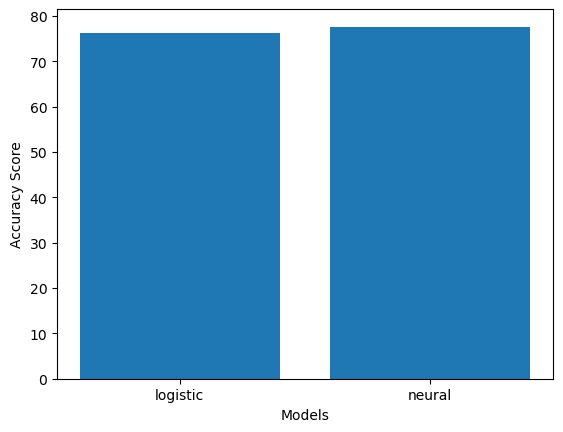
\includegraphics{./e2e_files/figure-pdf/cell-17-output-1.png}

}

\end{figure}

Here we have used accuracy for comparison. You can also use precision,
recall, or f1 score in a similar fashion for comparing models, depending
on the domain of prediction.

\hypertarget{step-17-save-your-best-model-for-production}{%
\subsection*{Step 17: Save your best model for
production}\label{step-17-save-your-best-model-for-production}}
\addcontentsline{toc}{subsection}{Step 17: Save your best model for
production}

The model you found to be the best performing one can be saved to the
disk so that you don't have to train your models every time you restart
Julia or you want to make predictions. We'll need three packages to save
a \texttt{scikit-learn} model: \texttt{PyCall}, \texttt{PyCallJLD}, and
\texttt{JLD}

\begin{Shaded}
\begin{Highlighting}[]
\ImportTok{using} \BuiltInTok{PyCall}\NormalTok{, }\BuiltInTok{JLD}\NormalTok{, }\BuiltInTok{PyCallJLD}
\FunctionTok{save}\NormalTok{(}\StringTok{"saved\_file.jld"}\NormalTok{, }\StringTok{"diabetic\_prediction"}\NormalTok{, best\_logistic\_model)}
\end{Highlighting}
\end{Shaded}

\begin{itemize}
\tightlist
\item
  The save function takes three arguments: the name of the file, the
  name you want to give to the model, the trained model.
\end{itemize}

To load a saved \texttt{scikit-learn} model, you can use the load
function:

\begin{Shaded}
\begin{Highlighting}[]
\NormalTok{logistic\_model }\OperatorTok{=} \FunctionTok{load}\NormalTok{(}\StringTok{"saved\_file.jld"}\NormalTok{, }\StringTok{"diabetic\_prediction"}\NormalTok{)}
\end{Highlighting}
\end{Shaded}

\begin{verbatim}
PyObject LogisticRegression(C=0.01, solver='newton-cg')
\end{verbatim}

Now let's check if our loaded model is working.

\begin{Shaded}
\begin{Highlighting}[]
\FunctionTok{predict}\NormalTok{(logistic\_model, X\_test)[}\FloatTok{1}\OperatorTok{:}\FloatTok{4}\NormalTok{]}
\end{Highlighting}
\end{Shaded}

\begin{verbatim}
4-element Vector{Any}:
 "No"
 "No"
 "No"
 "No"
\end{verbatim}


\backmatter

\end{document}
